\setdictum{%
  B-splines are not enough!%
}{%
  In a talk at the 2017 SIAM Conference on\\
  Computational Science and Engineering%
}
% SIAM CSE 2017, Minisymposium MS154 "Flooding the Cores--Computing Flooding
% Events on Modern Architecture--Part I of II",
% Craig Michoski, UT Austin,
% "Scaling at Exascale in Blended Isogeometric, Discontinuous
% Galerkin, and Particle-in-Cell Approaches"

\chapter{Hierarchical B-Splines and Sparse Grids}
\label{sec:20sparseGrids}

\todo{Write short intro to SGs? Overlap with Chap. 1?}

The aim of this chapter is to define hierarchical B-splines on sparse grids.
It is structured as follows:
\Cref{sec:21sparseGrids} provides a consistent notational framework
for the definition of sparse grids with general basis functions.
The reason not to employ specific bases such as the common hat functions
or B-splines of higher degrees is two-fold:
First, we will define various new ``flavors'' of B-splines,
which is easier if the basis is left open in the basic definitions.
Second, most of the statements and theorems that we will make in this
thesis will hold for general basis functions
(in some case with additional assumptions)
and not just for B-splines for example.
Next, \cref{sec:22bSplines} defines hierarchical B-splines for both
uniform and non-uniform knot sequences.
Finally, we will see in \cref{sec:23boundary} that the boundary behavior
of the classical uniform B-spline basis is problematic.
We will incorporate not-a-knot boundary conditions into the B-spline
basis to mitigate this issue.

\section{Hierarchical Bases and Sparse Grids}
\label{sec:21sparseGrids}

This section is, besides the derivation of sparse grids with
coarser boundary points in \cref{sec:213boundary},
a repetition of the definition of sparse grids with general basis functions.
Our notation and presentation will follow roughly
\cite{Pflueger10Spatially} and \cite{Garcke13Sparse}.
A more detailed introduction to sparse grids can be found in
\cite{Bungartz04Sparse}.



\subsection{Nodal Spaces}

\subsubsection{Univariate Case}

Let us first consider univariate functions
that are defined on the unit interval $[0, 1]$.
\newgsymbol{l}{$l$}{Level $\in \NN_0$}%
We discretize this domain by splitting it into $2^l$ equally sized segments,
where $l \in \NN_0$ is the \term{level}.
\newgsymbol{xli}{$x_{l,i}$}{Grid point $:= i \cdot h_l$}%
\newgsymbol{i}{$i$}{Index $= 0, \dotsc, 2^l$}%
\newgsymbol{hl}{$h_l$}{Mesh size $:= 2^{-l}$}%
The resulting $2^l + 1$ \term{grid points} are given by
\begin{equation}
  x_{l,i} := i \cdot h_l,\quad
  i = 0, \dotsc, 2^l,
\end{equation}
where $i$ is the \term{index} and $h_l := 2^{-l}$ is the \term{mesh size}.
\newgsymbol{phili}{$\varphi_{l,i}$}{%
  Hierarchical basis function of level $l$, index $i$%
}%
Every grid point is associated with a \term{basis function}
\begin{equation}
  \varphi_{l,i}\colon [0, 1] \to \RR.
\end{equation}
In this thesis, we assume $\varphi_{l,i}$ to be arbitrary,
satisfying required assumptions when needed and stated.
However, it helps for both the theory and the intuition to have a
specific example of basis functions in mind.
\newgsymbol{phili1}{$\varphi_{l,i}^1$}{Hat function of level $l$, index $i$}%
The so-called \term{hat functions} (linear B-splines), which are defined as
\begin{equation}
  \label{eq:hatFunctionUV}
  \varphi_{l,i}^1(x)
  := \max(1 - |x/h_l - i|, 0),
\end{equation}
are the most common choice for $\varphi_{l,i}$.
Here and in the following,
the superscript ``1'' is the degree of the linear B-spline and
is not to be read as an exponent.
We will generalize this notation to B-splines $\varphi_{l,i}^p$ of
arbitrary degrees $p$ (see \cref{sec:22bSplines}).

\newgsymbol{Vl}{$V_l$}{Nodal space of level $l$}%
\newgsymbol{span}{$\spn$}{Linear span (set of all linear combinations)}%
The \emph{nodal space} $V_l$ of level $l$
is defined as the linear span of all basis functions
$\varphi_{l,i}$:
\begin{equation}
  V_l := \spn\{\varphi_{l,i} \mid i = 0, \dotsc, 2^l\}.
\end{equation}
We assume that the functions $\varphi_{l,i}$ form a basis of $V_l$, i.e.,
every linear combination of these functions is unique.
\newgsymbol{fl}{$f_l$}{Interpolant of $f$ in $V_l$}%
\newgsymbol{ci}{$c_i$}{Coefficients of a linear combination}%
This ensures that for every objective function $f\colon [0, 1] \to \RR$,
there is a unique function $f_l\colon [0, 1] \to \RR$ such that
\begin{equation}
  \label{eq:interpFullGridUV}
  f_l
  = \sum_{i=0}^{2^l} c_i \varphi_{l,i},\quad
  \fa{i = 0, \dotsc, 2^l}{f_l(x_{l,i}) = f(x_{l,i})},
\end{equation}
for some $c_i \in \RR$.
In this case, $f_l$ is called \term{interpolant} of $f$ in $V_l$.
\newgsymbol{Vl1}{$V_l^1$}{Nodal piecewise linear space of level $l$}%
The nodal space $V_l^1$ is defined analogously as the span of the
hat functions $\varphi_{l,i}^1$.
It is the space of all linear splines,
that is, the space of all continuous functions on $[0, 1]$ that are
piecewise linear polynomials on $[x_{l,i}, x_{l,i+1}]$ for
$i = 0, \dotsc, 2^l - 1$.
The nodal hat function basis of level $3$
and a linear combination are shown in \cref{fig:nodalHat}.

\begin{figure}
  \subcaptionbox{%
    Basis functions $\varphi_{l,i}^1$ and grid points $x_{l,i}$
    \emph{(dots)}.%
  }[75mm]{%
    \includegraphics{nodalHat_1}%
  }%
  \hfill%
  \subcaptionbox{%
    Piecewise linear interpolant $f_l$ as a weighted sum
    of the nodal hat functions.%
  }[75mm]{%
    \includegraphics{nodalHat_2}%
  }%
  \caption{Univariate nodal hat functions of level $l = 3$.}
  \label{fig:nodalHat}
\end{figure}

\subsubsection{Multivariate Case}

\newgsymbol{d}{$d$}{Dimensionality $\in \NN$}%
For the multivariate case with $d \in \NN$ dimensions,
we proceed with the usual tensor product approach,
for which we replace all indices, points, and functions with
multi-indices, Cartesian products, and tensor products, respectively.
\newgsymbol{0!}{$\ß0$}{$(0, \dotsc, 0) \in \NN_0^d$}%
\newgsymbol{1!}{$\ß1$}{$(1, \dotsc, 1) \in \NN^d$}%
\newgsymbol{01!}{$[\ß0, \ß1]$}{%
  Unit hypercube $:= [0, 1]^d$%
}
\newgsymbol{l!}{$\ßl$}{Multivariate level $\in \NN_0^d$}%
\newgsymbol{norm1}{$\norm{\cdot}_1$}{1-norm $\norm{\ßx}_1 := \sum_{t=1}^d x_t$}%
Therefore, the domain is now $[\ß0, \ß1] := [0, 1]^d$,
which can be partitioned into
$\prod_{t=1}^d 2^{l_t} = 2^{\norm{\vec{l}}_1}$ equally sized hypercubes,
where $\ßl = (l_1, \dotsc, l_d) \in \NN_0^d$ is the $d$-dimensional level
and $\norm{\vec{l}}_1 := \sum_{t=1}^d l_t$ is the level sum.
\newgsymbol{xli!}{$\ßx_{\ßl,\ßi}$}{Multivariate grid point $:= \ßi \cdot \ßh_\ßl$}%
\newgsymbol{i!}{$\ßi$}{Multivariate index $= \ß0, \dotsc, \ß2^l$}%
\newgsymbol{i02l!}{$\ßi = \ß0, \dotsc, \ß2^l$}{%
  For all $\ßi$ with $0 \le i_t \le 2^{l_t}$ for all $t = 1, \dotsc, d$%
}%
The corners of the hypercubes are given by the grid points
\begin{equation}
  \label{eq:gridPointMultivariate}
  \ßx_{\ßl,\ßi} := \ßi \cdot \ßh_\ßl,\quad
  \ßi = \ß0, \dotsc, \ß2^{\ßl}.
\end{equation}
To allow for a somewhat intuitive and suggestive notation,
relations and operations with vectors (in bold face)
are to be read coordinate-wise in this thesis, unless stated otherwise.
Bold-faced numbers like $\ß0$ are defined to be the vector $(0, \dotsc, 0)$
in which every entry is equal to that number.
\newgsymbol{hl!}{$\ßh_\ßl$}{Multivariate mesh size $:= \ß2^{-\ßl}$}%
For example, \eqref{eq:gridPointMultivariate} is equivalent to
\begin{equation}
  \ßx_{\ßl,\ßi}
  := (i_1 h_{l_1},\; \dotsc,\; i_d h_{l_d}),\quad
  i_t = 0, \dotsc, 2^{l_t},\quad
  t = 1, \dotsc, d,
\end{equation}
with the $d$-dimensional mesh size
$\ßh_\ßl := \ß2^{-\ßl} = (h_{l_1}, \dotsc, h_{l_d})$.
\newgsymbol{phili!}{$\varphi_{\ßl,\ßi}$}{%
  Multivariate hierarchical basis function of level $\ßl$, index $\ßi$%
}%
Again, every grid point is associated with a basis function that is defined
as the tensor product of the univariate functions:%
\footnote{%
  Note that one could employ basis functions of different types in
  each dimension, for example B-splines of different degrees.
  For simplicity, we first restrict ourselves to the case of a single type
  for all dimensions, but we will treat the more general case in
  \todo{insert reference}.%
}
\begin{equation}
  \varphi_{\ßl,\ßi}\colon [\ß0, \ß1] \to \RR,\quad
  \varphi_{\ßl,\ßi}(\ßx)
  := \prod_{t=1}^d \varphi_{l_t,i_t}(x_t).
\end{equation}
\cref{fig:nodalHat2D} shows an example of a bivariate nodal hat function
$\varphi_{\ßl,\ßi}^1$.

\begin{figure}
  \includegraphics{nodalHat2D_1}%
  \caption{%
    Bivariate nodal hat function of level $\ßl = (2, 1)$ and
    index $i = (1, 1)$ as the tensor product of two univariate
    nodal hat functions.%
  }
  \label{fig:nodalHat2D}
\end{figure}

\newgsymbol{Vl!}{$V_\ßl$}{Multivariate nodal space of level $\ßl$}%
The multivariate nodal space $V_\ßl$ is defined analogously to
the univariate case:
\begin{equation}
  V_\ßl
  := \spn\{\varphi_{\ßl,\ßi} \mid \ßi = \ß0, \dotsc, \ß2^{\ßl}\}.
\end{equation}
\newgsymbol{phili1!}{$\varphi_{\ßl,\ßi}^1$}{%
  Multivariate hat function of level $\ßl$, index $\ßi$%
}%
\newgsymbol{Vl1!}{$V_\ßl^1$}{%
  Multivariate nodal piecewise linear space of level $\ßl$%
}%
\newgsymbol{ab!}{$[\ßa, \ßb]$}{%
  Hypercube $:= [a_1, b_1] \times \dotsb \times [a_d, b_d]$%
}%
In the case of hat functions $\varphi_{\ßl,\ßi}^1$,
the nodal space $V_\ßl^1$ is the $d$-linear spline space, i.e.,
the space of all continuous functions
on $[\ß0, \ß1]$ that are piecewise $d$-linear polynomials on
all hypercubes
\begin{equation}
  [\ßx_{\ßl,\ßi}, \ßx_{\ßl,\ßi+\ß1}]
  := [x_{l_1,i_1}, x_{l_1,i_1+1}] \times \dotsb \times
  [x_{l_d,i_d}, x_{l_d,i_d+1}],\quad
  \ßi = \ß0, \dotsc, \ß2^\ßl - \ß1.
\end{equation}
\newgsymbol{fl!}{$f_\ßl$}{Interpolant of $f$ in $V_\ßl$}%
\newgsymbol{ci!}{$c_\ßi$}{Coefficients of a linear combination}%
Analogously to \eqref{eq:interpFullGridUV},
we can interpolate objective functions $f\colon [\ß0, \ß1] \to \RR$
in the nodal space $V_\ßl$ with $f_\ßl\colon [\ß0, \ß1] \to \RR$ satisfying
\begin{equation}
  \label{eq:interpFullGridMV}
  f_\ßl
  = \sum_{\ßi=\ß0}^{\ß2^\ßl} c_\ßi \varphi_{\ßl,\ßi},\quad
  \fa{\ßi = \ß0, \dotsc, \ß2^\ßl}{f_\ßl(\ßx_{\ßl,\ßi}) = f(\ßx_{\ßl,\ßi})},
\end{equation}
where $c_\ßi \in \RR$ and
the sum is over all $\ßi = \ß0, \dotsc, \ß2^\ßl$.
\begin{lemma}[Linear independence of tensor products]
  \label{lemma:tensorProductLinearIndependence}
  The functions $\varphi_{\ßl,\ßi}$ ($\ßi = \ß0, \dotsc, \ß2^\ßl$)
  form a basis of $V_\ßl$, if the univariate functions
  $\varphi_{l_t,i_t}$ ($i_t = 0, \dotsc, 2^{l_t}$)
  form a basis of the univariate nodal space $V_{l_t}$
  for $t = 1, \dotsc, d$.
\end{lemma}
\begin{proof}
  \newgsymbol{!equiv}{$\equiv$}{%
    Equality of functions everywhere on their domain
    (e.g., $f \equiv 0$ means $f(x) = 0$ for all feasible $x$)%
  }%
  Assume that $c_\ßi \in \RR$ are chosen in \eqref{eq:interpFullGridMV}
  such that $f_\ßl \equiv 0$.
  Then for all $\ßi' = \ß0, \dotsc, \ß2^\ßl$,
  we can evaluate \eqref{eq:interpFullGridMV} at $\ßx_{\ßl,\ßi'}$ to obtain
  \begin{equation}
    \sum_{i_1=0}^{2^{l_1}}
    \left(\sum_{i_2=0}^{2^{l_2}} \dotsb
    \left(\sum_{i_d=0}^{2^{l_d}} c_\ßi \varphi_{l_d,i_d}(x_{l_d,i_d'})\right) \dotsb
    \varphi_{l_2,i_2}(x_{l_2,i_2'})\right) \varphi_{l_1,i_1}(x_{l_1,i_1'})
    = 0.
  \end{equation}
  We apply the linear independence in 1D ($x_1$ direction) to conclude that
  the sum over $i_2$ must vanish.
  Repeating this argument for all dimensions, we infer that $c_\ßi = 0$
  for all $\ßi = \ß0, \dotsc, \ß2^\ßl$,
  implying the linear independence of the functions $\varphi_{\ßl,\ßi}$.
\end{proof}
\newgsymbol{Omegal!}{$\Omega_\ßl$}{Set of full grid points of level $\ßl$}%
The lemma is equivalent to the statement that the coefficients $c_\ßi \in \RR$
exist for every objective function $f$ and are uniquely determined by
the values at the grid points
\begin{equation}
  \Omega_\ßl
  := \{\ßx_{\ßl,\ßi} \mid \ßi = \ß0, \dotsc, \ß2^{\ßl}\}.
\end{equation}
\newgsymbol{n}{$n$}{Level $\in \NN_0$ of full or sparse grid}
A common choice for the level $\ßl$ is $n \cdot \ß1$ for some $n \in \NN_0$.
\newgsymbol{Vnd}{$V_{n,d}$}{%
  Multivariate nodal space
  $:= V_{n \cdot \ß1}$ of level $n$ with dimensionality $d$%
}%
\newgsymbol{Vnd1}{$V_{n,d}^1$}{%
  Multivariate nodal piecewise linear space
  $:= V_{n \cdot \ß1}^1$ of level $n$ with dimensionality $d$%
}%
In this case, we replace ``$\ßl$'' in the subscripts with ``$n,d$''
(for example, $V_{n,d} := V_{n \cdot \ß1}$).
\newgsymbol{fnd1}{$f_{n,d}^1$}{Full grid interpolant $\in V_{n,d}^1$ of $f$}%
\newgsymbol{||.||L2}{$\norm{\cdot}_{L^2}$}{%
  $L^2$ norm $\norm{f}_{L^2} := \sqrt{\int_\Omega f(x)^2 \dx}$
  for a function $f\colon \Omega \to \RR$%
}
\newgsymbol{O}{$\calO(f(x))$}{Big-$\calO$ Landau notation}%
For the hat function basis $\varphi_{l,i}^1$,
it can be shown that the $L^2$ interpolation error of the interpolant
$f_{n,d}^1$ is given by
\begin{equation}
  \norm{f - f_{n,d}^1}_{L^2} = \calO(h_n^2),
\end{equation}
i.e., the order of the interpolation error is quadratic in the mesh size
\cite{Hoellig13Approximation,Bungartz04Sparse}.



\subsection{Hierarchical Subspaces}

\newgsymbol{dim}{$\dim$}{Vector space dimension}%
\newgsymbol{|.|}{$|\cdot|$}{%
  Absolute value of a scalar or the number of elements of a set%
}%
The dimension of the nodal space $V_\ßl$ is given by
\begin{equation}
  \label{eq:dimensionFG}
  \dim V_\ßl
  = |\Omega_\ßl|
  = \prod_{t=1}^d (2^{l_t} + 1).
\end{equation}
If we choose the same level $n \in \NN_0$ in all dimensions,
then the dimension of $V_{n,d}$ and the
number of grid points grow at least as fast as
$2^{nd} = (h_n^{-1})^d$.
This exponential dependency between $\dim V_{n,d}$ and $d$ is known as the
\term{curse of dimensionality}.
The curse makes interpolation on $V_\ßl$ computationally infeasible
for dimensionalities $d > 4$,
as we would have to calculate and store $\dim V_\ßl$ coefficients $c_\ßi$.%
\footnote{%
  The number of necessary basis evaluations to evaluate the interpolant once
  would not be as large, as most types of basis functions
  (like hat functions $\varphi_{l,i}^1$ and higher-order B-splines)
  are locally supported.%
}

\subsubsection{Hierarchical Splitting in the Univariate Case}

In order to reduce the computational effort,
we first split $V_\ßl$ into smaller subspaces and then identify
which subspaces are most important and which subspaces can be omitted
at the cost of a slightly larger error.
In the univariate case, the key observation is that a grid point of a level $l$
can be written as a grid point of a higher level $l'$:
\begin{equation}
  x_{l,i} = x_{l',i'},\quad
  l' \ge l,\quad
  i' = 2^{l'-l} i.
\end{equation}
\newgsymbol{xor}{$\xor$}{Bitwise ``exclusive or''}%
Conversely, this implies that every grid point $x_{l,i}$ of level $l \ge 1$
can be uniquely written
as a grid point of a coarser level $l'$ and an odd index $i'$:
\begin{equation}
  x_{l,i} = x_{l',i'},\quad
  l' = l - \left[\log_2(\xor(i, i-1) + 1) - 1\right],\quad
  i' = i/2^{l-l'},
\end{equation}
% https://mathoverflow.net/a/29973
where $\xor$ is the bitwise ``exclusive or'' function.
The term in brackets is the exponent of the
highest power of two that divides $i$.
\newgsymbol{u!}{$\dotcup$}{%
  Disjoint union of sets (union where the pairwise intersection of
  the joined sets is empty)%
}%
\newgsymbol{Il}{$I_l$}{Set of (odd) indices for hierarchical basis functions}%
This implies that $\Omega_l$ decomposes into
\begin{equation}
  \Omega_l
  = \bigdotcup_{l'=0}^l \{x_{l',i'} \mid i' \in I_{l'}\},\quad
  I_{l'} :=
  \begin{cases}
    \{i = 0, \dotsc, 2^{l'} \mid \text{$i$ odd}\},&l' > 0,\\
    \{0, 1\},&l' = 0,
  \end{cases}
\end{equation}
where $\dotcup$ indicates the disjoint union.
\newgsymbol{Wl}{$W_l$}{Hierarchical subspace of level $l$}%
We call the spaces spanned by the basis functions that correspond to the
joined sets \term{hierarchical subspaces} $W_l$:
\begin{equation}
  W_l
  := \spn\{\varphi_{l,i} \mid i \in I_l\}.
\end{equation}

\newgsymbol{oplus}{$\oplus$}{%
  Direct sum of vector spaces (vector space sum in which the dimension of
  the sum equals the sum of the summands' dimensions)%
}%
For the hat function basis $\varphi_{l,i}^1$ and other basis types,
one can prove that the corresponding nodal space
decomposes into the direct sum of all
hierarchical subspaces of coarser levels or the same level, i.e.,
\begin{equation}
  \label{eq:hierSplittingUV}
  V_l
  = \bigoplus_{l'=0}^l W_{l'},
\end{equation}
Here, the direct sum $\oplus$ is
the normal vector space sum with the additional indication
that the dimension of the sum $\sum_{l'=0}^l W_{l'}$ is the sum
of the dimensions of the summands $W_{l'}$
(analogously to $|\Omega_l| = \sum_{l'=0}^l |\Omega_{l'}|$,
where $\Omega_l$ is the disjoint union of the sets $\Omega_{l'}$).
In general, \eqref{eq:hierSplittingUV} may not be true.
The following lemma provides a characterization,
which can be used to prove \eqref{eq:hierSplittingUV} for hat functions.
The hierarchical hat function basis is shown in \cref{fig:hierarchicalHat}.

\begin{figure}
  \subcaptionbox{%
    Basis functions $\varphi_{l,i}^1$ and grid points $x_{l,i}$
    \emph{(dots)}.
    The domain is the unit interval $[0, 1]$.%
  }[75mm]{%
    \includegraphics{hierarchicalHat_1}%
  }%
  \hfill%
  \subcaptionbox{%
    Piecewise linear interpolant $f_l$ as a weighted sum
    of the hierarchical hat functions \emph{(stacked)}.
    The two boundary functions are combined to a single function
    \emph{\textcolor{C0}{(blue)}} for simplicity.%
  }[75mm]{%
    \includegraphics{hierarchicalHat_2}%
  }%
  \caption{Univariate hierarchical hat functions of level $l' = 0, \dotsc, 3$.}
  \label{fig:hierarchicalHat}
\end{figure}

\begin{lemma}[Hierarchical splitting characterization]
  \label{lemma:hierSplittingUV}
  Equivalent to relation \eqref{eq:hierSplittingUV} is the satisfaction of
  both of the following conditions:
  \begin{itemize}
    \item
    The hierarchical subspaces $W_{l'}$ ($l' \le l$) are subspaces of $V_l$.
    
    \item
    The hierarchical functions
    $\varphi_{l',i'}$ ($l' \le l$, $i' \in I_{l'}$) are linearly independent.
  \end{itemize}
\end{lemma}
\begin{proof}
  The first condition is equivalent to $\sum_{l'=0}^l W_{l'} \subset V_l$.
  The second condition is equivalent to
  $\dim \sum_{l'=0}^l W_{l'} = \sum_{l'=0}^l \dim W_{l'}$,
  i.e., to the directness of the sum.
  Therefore, the logical conjunction of both is equivalent to
  $\bigoplus_{l'=0}^l W_{l'} \subset V_l$.
  If the sum is direct,
  the dimension of the sum is equal to $2 + \sum_{l'=1}^l 2^{l'-1} = 2^l + 1$
  (due to $\dim W_{l'} = |I_{l'}| = 2^{l'-1}$ for $l' > 0$ and
  $\dim W_{l'} = 2$ for $l' = 0$),
  which is also the dimension of $V_l$.
  The only subspace of $V_l$ that has the same dimension as $V_l$ is $V_l$ itself,
  so we infer $\bigoplus_{l'=0}^l W_{l'} = V_l$.
\end{proof}
\begin{corollary}
  The hierarchical splitting \eqref{eq:hierSplittingUV}
  holds for the hat function basis.
\end{corollary}
\begin{proof}
  The first condition of \cref{lemma:hierSplittingUV}
  is satisfied as piecewise linear splines of level $l'$
  are also piecewise linear splines of higher levels $l \ge l'$.
  The linear independence for the second condition can be proved by induction
  over $l$:
  If a linear combination of $\varphi_{l',i'}^1$ ($l' \le l$, $i' \in I_{l'}$)
  vanishes everywhere, then the coefficients of level $l$ must be zero,
  as otherwise the basis functions $\varphi_{l,i'}^1$ ($i' \in I_l$) would
  introduce kinks at $x_{l,i'}$, which the zero function does not have.
  This means that we have a zero linear combination of $\varphi_{l',i'}^1$ for
  $l' \le l - 1$, $i' \in I_{l'}$,
  and by the induction hypothesis, the other coefficients also vanish.
\end{proof}

\subsubsection{Hierarchical Splitting in the Multivariate Case}

\newgsymbol{Wl!}{$W_\ßl$}{Multivariate hierarchical subspace of level $\ßl$}%
\newgsymbol{Il!}{$I_\ßl$}{%
  Set $:= I_{l_1} \times \dotsb \times I_{l_d}$ of
  (odd) multivariate indices for hierarchical basis functions%
}%
Multivariate hierarchical subspaces of level $\ßl$
are defined analogously to the univariate case:
\begin{equation}
  W_\ßl
  := \spn\{\varphi_{\ßl,\ßi} \mid \ßi \in I_\ßl\},\quad
  I_\ßl
  := I_{l_1} \times \dotsb \times I_{l_d}.
\end{equation}
The splitting \eqref{eq:hierSplittingUV} can now be generalized to the
multivariate case:
\begin{equation}
  \label{eq:hierSplittingMV}
  V_\ßl
  = \bigoplus_{\ßl'=0}^\ßl W_{\ßl'},
\end{equation}
Again, this relation does not hold in general.
A multivariate counterpart of \cref{lemma:hierSplittingUV} can be used
to prove that \eqref{eq:hierSplittingMV} holds if
the corresponding 1D relation \eqref{eq:hierSplittingUV} holds for all dimensions:
\begin{lemma}[Multivariate hierarchical splitting characterization]
  \label{lemma:hierSplittingMV}
  Equivalent to relation \eqref{eq:hierSplittingMV} is the satisfaction of
  both of the following conditions:
  \begin{itemize}
    \item
    The hierarchical subspaces $W_{\ßl'}$ ($\ßl' \le \ßl$) are subspaces of $V_\ßl$.
    
    \item
    The basis functions $\varphi_{\ßl',\ßi'}$ ($\ßl' \le \ßl$, $\ßi' \in I_{\ßl'}$)
    are linearly independent.
  \end{itemize}
\end{lemma}
\begin{proof}
  If the sum is direct, then its dimension is given by
  \begin{equation}
    \dim \sum_{\ßl'=0}^\ßl W_{\ßl'}
    = \sum_{l_1'=0}^{l_1} \dotsb \sum_{l_d'=0}^{l_d}
    \prod_{t=1}^d \dim W_{l_t'}
    = \prod_{t=1}^d \sum_{l_t'=0}^{l_t} \dim W_{l_t'}
    = \prod_{t=1}^d (2^{l_t} + 1)
    = \dim V_\ßl
  \end{equation}
  using \eqref{eq:dimensionFG}.
  The rest is analogous to the proof of \cref{lemma:hierSplittingUV}.
\end{proof}
\begin{proposition}
  If univariate splitting \eqref{eq:hierSplittingUV} holds for every dimension,
  then the multivariate splitting \eqref{eq:hierSplittingMV} holds as well.
\end{proposition}
\begin{proof}
  We check the two conditions of \cref{lemma:hierSplittingMV}
  given the two univariate conditions of \cref{lemma:hierSplittingUV}:
  \begin{enumerate}
    \item
    The hierarchical basis functions $\varphi_{\ßl',\ßi'}$
    of $W_{\ßl'}$ ($\ßl' \le \ßl$, $\ßi' \in I_{\ßl'}$) are tensor products
    of functions $\varphi_{l_t',i_t'}$.
    According to the first condition of \cref{lemma:hierSplittingUV},
    each $\varphi_{l_t',i_t'}$ can be written as a linear combination of
    the nodal basis $\varphi_{l_t,i_t}$ ($i_t = 0, \dotsc, 2^{l_t}$).
    We can expand the tensor product to a linear combination
    of tensor products of the univariate nodal basis functions.
    Therefore, $\varphi_{\ßl',\ßi'}$ is a linear combination of
    multivariate nodal functions, i.e., $\varphi_{\ßl',\ßi'} \in V_\ßl$.
    As this is true for all $\ßi' \in I_{\ßl'}$, we obtain $W_{\ßl'} \subset V_\ßl$.
    
    \item
    The linear independence of the hierarchical functions $\varphi_{\ßl',\ßi'}$
    ($\ßl' \le \ßl$, $\ßi' \in I_{\ßl'}$) can be shown completely analogously
    to the proof of \cref{lemma:tensorProductLinearIndependence}.\qedhere
  \end{enumerate}
\end{proof}
\begin{corollary}
  The multivariate hierarchical splitting \eqref{eq:hierSplittingMV}
  holds for the hat function basis.\qed
\end{corollary}



\subsection{Sparse Grids}

The idea of sparse grids is to use the
hierarchical splitting \eqref{eq:hierSplittingUV}
to keep only the most ``important'' hierarchical subspaces,
omitting the remaining ones.
There are three main ``flavors'' of sparse grids:
regular, dimensionally adaptive, and spatially adaptive.

\subsubsection{Regular Sparse Grids}

To assess the importance of a subspace, we consider again the
interpolant $f_\ßl \in V_\ßl$ of a function $f\colon [\ß0, \ß1] \to \RR$.
According to the splitting \eqref{eq:hierSplittingMV}, the interpolant can
be written as
\begin{equation}
  \label{eq:interpHierFullGrid}
  f_\ßl
  = \sum_{\ßl'=0}^\ßl \sum_{\ßi'=\ß0}^{\ß2^{\ßl'}}
  \alpha_{\ßl',\ßi'} \varphi_{\ßl',\ßi'},\quad
  \fa{\ßi = \ß0, \dotsc, \ß2^\ßl}{f_\ßl(\ßx_{\ßl,\ßi}) = f(\ßx_{\ßl,\ßi})}.
\end{equation}
\newgsymbol{alphali!}{$\alpha_{\ßl,\ßi}$}{%
  Hierarchical surpluses (coefficients of a linear combination of hierarchical
  basis functions)%
}%
The coefficients $\alpha_{\ßl',\ßi'}$ with respect to the hierarchical basis
$\varphi_{\ßl',\ßi'}$ are the \term{hierarchical surpluses}.
When using the hat function basis $\varphi_{\ßl,\ßi}^1$,
one can prove the following representation
for the corresponding surpluses \cite{Bungartz04Sparse}:
\begin{equation}
  \alpha_{\ßl,\ßi}
  = (-1)^d 2^{-\norm{\ßl+\ß1}_1}
  \int_\ß0^\ß1 \varphi_{\ßl,\ßi}^1(\ßx)
  \frac{\partialdiff^{2d}}{\partialdiff x_1^2 \dotsb \partialdiff x_d^2}
  f(\ßx) \diff{}\ßx,
\end{equation}
if $\ßl \ge \ß1$ and
$f$ is twice continuously differentiable in every dimension simultaneously,
i.e.,
$\frac{\partialdiff^{2d}}{\partialdiff x_1^2 \dotsb \partialdiff x_d^2} f$
exists and is continuous.%
\footnote{%
  Again, the notation implies that the integration domain is
  the hypercube $[\ß0, \ß1]$.%
}\multiplefootnoteseparator%
\footnote{%
  The statement is even valid for functions in the Sobolev space
  $H_\mathrm{mix}^2([\ß0, \ß1])$ with dominating mixed derivative,
  as its proof mainly relies on integration by parts
  \cite{Bungartz04Sparse}.%
}
%This equation provides a direct relation between the hat function surpluses
%and the second mixed derivative of the objective function, which has
%two consequences.
%First, the absolute value of the surpluses is large in regions where
%the absolute value of the second mixed derivative is large, i.e.,
%where the objective function oscillates strongly.
%Second, the absolute surpluses decay with
%increasing level $\ßl$ as both the factor
%$2^{-\norm{\ßl+\ß1}_1}$ and the size of the support of $\varphi_{\ßl,\ßi}$
%are decreasing.
Consequently, the contribution of the summand of level $\ßl$
can be estimated by
\begin{equation}
  \label{eq:componentEstimation}
  \bignorm{\sum_{\ßi'=\ß0}^{\ß2^{\ßl'}}
  \alpha_{\ßl',\ßi'} \varphi_{\ßl',\ßi'}^1}_{L^2}
  \le 3^{-d} \cdot 2^{-2 \norm{\ßl}_1} \cdot
  \bignorm{\frac{\partialdiff^{2d}}{
      \partialdiff x_1^2 \dotsb \partialdiff x_d^2
  } f}_{L^2}
\end{equation}
for the hat function surpluses $\alpha_{\ßl',\ßi'}$ \cite{Bungartz04Sparse}.

Equation \eqref{eq:componentEstimation} motivates to omit those summands
from the sum \eqref{eq:interpHierFullGrid} whose level sum $\norm{\ßl}_1$
exceeds a certain value $n \in \NN_0$.
More formally, the selection of the relevant subspaces can be formulated as a
continuous knapsack problem.
\newgsymbol{Vnds}{$V_{n,d}^\sparse$}{%
  Regular sparse grid space of level $n$ with dimensionality $d$%
}%
\newgsymbol{Omegands}{$\Omega_{n,d}^\sparse$}{%
  Set of regular sparse grid points of level $n$ with dimensionality $d$%
}%
The resulting function space and grid point set
\begin{equation}
  V_{n,d}^\sparse
  := \bigoplus_{\norm{\ßl}_1 \le n} W_{\ßl},\qquad
  \Omega_{n,d}^\sparse
  := \bigdotcup_{\norm{\ßl}_1 \le n}
  \{\ßx_{\ßl,\ßi} \mid \ßi \in I_{\ßl}\}
\end{equation}
are called \term{regular sparse grid space} and
\term{regular sparse grid} of level $n$, respectively.
To better distinguish the different grids,
we call the nodal spaces and grids \term{full grids}.
Although sparse grids have been motivated using the hat function
basis $\varphi_{\ßl,\ßi}^1$,
we generalize the definition to arbitrary bases $\varphi_{\ßl,\ßi}$.
\Cref{fig:regularSG} shows the construction of a
regular sparse grid in two dimensions.

\begin{figure}
  \subcaptionbox{%
    Hierarchical splitting and subspace selection.
    The rectangles indicate the support of the
    bivariate hat basis functions.%
  }[85mm]{%
    \includegraphics{sg_1}%
  }%
  \hfill%
  \begin{minipage}[b]{65mm}
    \subcaptionbox{%
      Full grid obtained by adding all subspaces of level $\ßl \le n \cdot \ß1$.%
    }[65mm]{%
      \includegraphics{sg_2}%
    }\\[5mm]%
    \subcaptionbox{%
      Regular sparse grid obtained by adding all subspaces
      whose level $\ßl$ satisfies $\norm{\ßl}_1 \le n$
      \emph{\textcolor{mittelblau}{(blue)}}.%
    }[65mm]{%
      \includegraphics{sg_3}%
    }%
  \end{minipage}
  \caption{Regular sparse grid of level $n = 3$ in two dimensions.}
  \label{fig:regularSG}
\end{figure}

\newgsymbol{Omegad}{$\bndry{\Omega}$}{%
  Boundary of the domain $\Omega \subset \RR^d$%
}%
One can prove that for homogeneous boundary conditions
$f|_{\bndry{[\ß0,\ß1]}} \equiv 0$,
the number of required inner grid points
($\ßx_{\ßl,\ßi} \in \Omega_{n,d}^\sparse$ where $\ßl \ge \ß1$)
grows like $\calO(h_n^{-1} (\log_2 h_n^{-1})^{d-1})$
\cite{Bungartz04Sparse}, which is much less than
the corresponding number $\calO((h_n^{-1})^d)$ in the full grid case
(see \eqref{eq:dimensionFG}).
In particular, the exponential dependency on the dimensionality $d$
has vanished.
\newgsymbol{fnds1}{$f_{n,d}^{\sparse,1}$}{%
  Sparse grid interpolant $\in V_{n,d}^{\sparse,1}$ of $f$%
}%
The corresponding $L^2$ error of the sparse grid interpolant
$f_{n,d}^{\sparse,1}$ using hat functions
(still assuming homogeneous boundary conditions) decays like
\begin{equation}
  \norm{f - f_{n,d}^{\sparse,1}}_{L^2} = \calO(h_n^2 (\log_2 h_n^{-1})^{d-1}),
\end{equation}
which is only slightly worse than the full grid error by the factor of
$(\log_2 h_n^{-1})^{d-1}$ \cite{Bungartz04Sparse}.

\subsubsection{Dimensionally Adaptive Sparse Grids}

The idea of dimensional adaptivity is to spend more grid
points along specific dimensions depending on the objective function.
Different criteria for the choice of dimensions exists,
for example the absolute value of the linear hierarchical surpluses
or the ANOVA decomposition.
\todo{not sure about that one}
To incorporate dimensional adaptivity into sparse grids,
one has to generalize the symmetric
choice of subspaces in the definition of regular sparse grids
to allow for an asymmetric preference.
\newgsymbol{Vs}{$V^\sparse$}{%
  Arbitrary sparse grid space (possibly spatially adaptive)%
}%
\newgsymbol{Omegas}{$\Omega^\sparse$}{%
  Arbitrary sparse grid (possibly spatially adaptive)%
}%
\newgsymbol{L}{$L$}{Finite subset $L \subset \NN_0^d$ of levels}%
Generally, function spaces $V^\sparse$ and grid sets $\Omega^\sparse$
of \term{dimensionally adaptive sparse grids} have the form
\begin{equation}
  V^\sparse
  = \bigoplus_{\ßl \in L} W_\ßl,\qquad
  \Omega^\sparse
  = \bigdotcup_{\ßl \in L} \{\ßx_{\ßl,\ßi} \mid \ßi \in I_\ßl\},
\end{equation}
where $L$ is a \term{downward closed} set, i.e.,
a finite subset $L \subset \NN_0^d$
for which $\forall_{\ßl \in L} \fa{\ßl' \le \ßl}{\ßl' \in L}$.
Regular sparse grids are a special case by setting
$L = \{\ßl \in \NN_0^d \mid \norm{\ßl}_1 \le n\}$.

The key advantage of dimensionally adaptive sparse grids over
spatially adaptive approaches lies in the
so-called \term{combination technique}.
\newgsymbol{cli!}{$c_{\ßl,\ßi}$}{%
  Interpolation coefficients for the full grid $V_\ßl$%
}%
For regular sparse grids, one can show that the sparse grid interpolant
$f_{n,d}^\sparse$ can be written as
\begin{equation}
  \label{eq:combiTechnique}
  f_{n,d}^\sparse
  = \sum_{q=0}^{d-1} (-1)^q \binom{d-1}{q} \sum_{\norm{\ßl}_1 = n-q}
  \sum_{\ßi=\ß0}^{\ß2^\ßl} c_{\ßl,\ßi} \varphi_{\ßl,\ßi},
\end{equation}
where the $c_{\ßl,\ßi} \in \RR$ ($\ßi = \ß0, \dotsc, \ß2^\ßl$)
are the interpolation coefficients on the full grid of level $\ßl$, i.e.,
$\fa{\ßi' = \ß0, \dotsc, \ß2^\ßl}{%
  \sum_{\ßi=\ß0}^{\ß2^\ßl} c_{\ßl,\ßi} \varphi_{\ßl,\ßi}(\ßx_{\ßl,\ßi'})
  = f(\ßx_{\ßl,\ßi'})%
}$ \cite{Smolyak63Quadrature,Zenger91Sparse}.
For general dimensionally adaptive sparse grids, a similar formula exists
\cite{Wasilkowski95Explicit}.
The combination formula \eqref{eq:combiTechnique},
which is visualized in \cref{fig:combinationTechnique}, splits the
sparse grid interpolant into a weighted sum of full grid interpolants.
In applications, each grid can be processed in parallel,
drastically speeding up computations like the solution of
partial differential equations (\pde{}s).
In addition, existing software working with nodal bases do not have to be
rewritten in terms of implementing hierarchical functions,
which means that combination technique allows sparse grids to be employed
in a minimally invasive way.

\begin{figure}
  \includegraphics{sg_4}%
  \caption{%
    The combination technique combines nodal subspaces in a weighted
    sum to form a regular sparse grid space of level $n = 3$ in two dimensions.
    The red subspaces ($q = 1$ in \eqref{eq:combiTechnique})
    are subtracted from the sum of the green subspaces ($q = 0$).%
  }
  \label{fig:combinationTechnique}
\end{figure}

\subsubsection{Spatially Adaptive Sparse Grids}

Dimensional adaptivity does not suffice to resolve local features of the
objective function.
Especially in some applications, it is crucial for the
interpolant to be highly accurate in specific regions of the domain.
For instance in optimization, it is not necessary to have a small global
interpolation error, but rather high accuracy near the optima is important.

This can be achieved by \term{spatially adaptive sparse grids},
on which this thesis focuses.
\newgsymbol{K}{$K$}{Finite set of level-index pairs $(\ßl,\ßi)$}%
In the most general form, their function spaces and grid sets have the form
\begin{equation}
  V^\sparse
  = \spn\{\varphi_{\ßl,\ßi} \mid (\ßl,\ßi) \in K\},\qquad
  \Omega^\sparse
  = \{\ßx_{\ßl,\ßi} \mid (\ßl,\ßi) \in K\},
\end{equation}
where $K$ is a finite set of level-index pairs $(\ßl,\ßi)$
with $\ßl \in \NN_0^d$ and $\ßi \in I_\ßl$.
Often, one has to make specific assumptions about $K$ in order for
sparse grid algorithms to work correctly.
\newgsymbol{et!}{$\ße_t$}{$t$-th unit vector $(0, \dotsc, 0, 1, 0, \dotsc, 0)$}%
For example for hat functions $\varphi_{\ßl,\ßi}^1$, the grid should contain
the hierarchical ancestors of every grid point:
\begin{equation}
  \label{eq:hierAncestors}
  \forall_{(\ßl,\ßi) \in K}
  \fa{\{t = 1, \dotsc, d \mid l_t \ge 1\}}{(\ßl',\ßi') \in K},\quad
  \ßl' := \ßl - \ße_t,\quad
  i_{t'}' :=
  \begin{cases}
    2 \lfloor i_t/4 \rfloor + 1,&t = t',\\
    i_{t'},&t \not= t',
  \end{cases}
\end{equation}
where $\ße_t$ is the $t$-th unit vector and $t' = 1, \dotsc, d$.
If \eqref{eq:hierAncestors} is not met, the so-called
unidirectional principle, which is used for instance to efficiently calculate
hierarchical surpluses, does not work.
However, as we will see, the unidirectional principle cannot be applied
to B-splines of general degree, even if \eqref{eq:hierAncestors} is satisfied.
Therefore, for most of our considerations, we will not restrict the
choice of $K$.

\begin{figure}
  \subcaptionbox{%
    Hierarchical splitting and grid point selection.
    The rectangles indicate again the support of the
    bivariate hat basis functions.%
  }[85mm]{%
    \includegraphics{sg_5}%
  }%
  \hfill%
  \subcaptionbox{%
    Resulting spatially adaptive sparse grid.%
  }[65mm]{%
    \includegraphics{sg_6}%
  }%
  \caption{%
    Spatially adaptive sparse grid in two dimensions.
    More grid points were generated in the top right corner,
    which can help to resolve fine oscillations of the objective function.%
  }
  \label{fig:spatiallyAdaptiveSG}
\end{figure}

\subsection{Boundary Treatment}
\label{sec:213boundary}

One issue of regular sparse grids $\Omega_{n,d}^\sparse$ as we have defined them
is that the number of grid points still grows very fast
with the level $n$ and the dimensionality $d$.
This is mainly because the finest mesh size $h_n$ on the
boundary of the domain $[\ß0, \ß1]$ is finer than
the finest mesh size $h_{n-d+1}$ that can be found in the interior.
\newgsymbol{Omegaso}{$\interior{\Omega}^\sparse$}{%
  Interior grid points $:= \Omega^\sparse \cap \openinterval{\ß0, \ß1}$
  for a finite set $\Omega^\sparse \subset [\ß0, \ß1]$ of grid points%
}%
\newgsymbol{01!}{$\openinterval{0, 1}$}{%
  Open unit interval $:= \{x \in \RR \mid 0 < x < 1\}$%
}%
\newgsymbol{01o!}{$\openinterval{\ß0, \ß1}$}{%
  Open unit hypercube $:= \openinterval{0, 1}^d$%
}%
If we define $\interior{\Omega}_{n,d}^\sparse$ as the set of
interior grid points in $\Omega_{n,d}^\sparse$, i.e.,%
\footnote{%
  Note that in the literature,
  the regular sparse grid space of level $n$ without boundary points is often
  defined via $\norm{\ßl}_1 \le n + d - 1$ to ensure that the finest mesh size
  is given by $h_n$.
  In our notation, this corresponds to $\interior{\Omega}_{n+d-1,d}^\sparse$.%
}
\begin{equation}
  \interior{\Omega}_{n,d}^\sparse
  := \Omega_{n,d}^\sparse \cap \openinterval{\ß0, \ß1}
  = \{\ßx_{\ßl,\ßi} \in \Omega_{n,d}^\sparse \mid \ßl \ge \ß1\},
\end{equation}
then the following relation about the number of grid points
of $\Omega_{n,d}^\sparse$ can be shown:
\begin{lemma}[Number of grid points of $\Omega_{n,d}^\sparse$]
  \label{lemma:numberOfGridPointsBoundary}
  \setlength{\abovedisplayskip}{0pt}
  \begin{equation}
    |\Omega_{n,d}^\sparse|
    = \sum_{q=0}^d 2^q \binom{d}{q} |\interior{\Omega}_{n+q,d-q}^\sparse|
  \end{equation}
\end{lemma}
\begin{proof}
  See \cite{Bungartz04Sparse}.
\end{proof}
Here, we define $0$-dimensional grids to contain exactly one grid point
(the empty tuple).
The number of interior grid points can be calculated as follows:
\begin{lemma}[Number of grid points of $\interior{\Omega}_{n,d}^\sparse$]
  \label{lemma:numberOfGridPointsInterior}
  \setlength{\abovedisplayskip}{0pt}
  \begin{equation}
    |\interior{\Omega}_{n,d}^\sparse|
    = \sum_{q=0}^{n-d} 2^q \binom{d-1+q}{d-1}
  \end{equation}
\end{lemma}
\begin{proof}
  See \cite{Bungartz04Sparse}.
\end{proof}

Intuitively, \cref{lemma:numberOfGridPointsBoundary} splits the sparse grid
$\Omega_{n,d}^\sparse$ into lower-dimensional sparse grids
$\interior{\Omega}_{n+q,d-q}^\sparse$ without boundary points.
The factor $2^q \binom{d}{q}$ is the number of $(d-q)$-dimensional faces
of the $d$-dimensional unit hypercube.
For example, the 3D cube decomposes into
$2^0 \binom{3}{0} = 1$ interior cube $\openinterval{0, 1}^3$,
$2^1 \binom{3}{1} = 6$ sides ($2$-dimensional faces)
like $\openinterval{0, 1}^2 \times \{0\}$,
$2^2 \binom{3}{2} = 12$ edges ($1$-dimensional faces)
like $\openinterval{0, 1} \times \{(0, 0)\}$, and
$2^3 \binom{3}{3} = 8$ corners ($0$-dimensional faces)
like $(0, 0, 0)$.
On each of these $(d-q)$-dimensional faces,
the sparse grid $\Omega_{n,d}^\sparse$ contains
the interior of a sparse grid of level $n + q$,
the size of which grows like $\calO(2^{n+q} n^{d-q-1})$.
As the number of boundary faces increases exponentially
with the dimensionality $d$,
the size of $\Omega_{n,d}^\sparse$ quickly exhausts the available
computational memory.
There are mainly two solutions to deal with this issue.

\subsubsection{Sparse Grids with Coarser Boundaries}

The first solution is to insert the boundary level functions and grid points
at a finer level than $0$.
A popular choice is the insertion at level $1$, which corresponds to
\begin{equation}
  \label{eq:sparseGridB1}
  \Omega_{n,d}^{\sparse(1)}
  := \bigdotcup_{\ßl \in L_{n,d}^{\sparse(1)}}
  \{\ßx_{\ßl,\ßi} \mid \ßi \in I_\ßl\},\quad
  L_{n,d}^{\sparse(1)}
  := \{\ßl \in \NN_0^d \mid \norm{\vecmax(\ßl, \ß1)}_1 \le n\},
\end{equation}
where $\vec{\max}$ is to be read coordinate-wise as usual.
This choice is equivalent to treating $0$-level components as level $1$
in the subspace selection.
This ensures that the finest mesh sizes in interior of $[\ß0, \ß1]$ and
its boundary coincide to be $h_{n-d+1}$, which reduces the number of grid points
on the boundary significantly.

Another solution that can be found in the literature about sparse grids with
hat functions is (in the univariate case)
to start with the constant function on level $0$ with
corresponding grid point $0.5$,
then employ the two boundary functions and points on level $1$,
and finally proceed as usual for the finer levels $\ge 2$.
Apart from a constant shift in the level of the resulting sparse grids,
this is equivalent to inserting the boundary functions and points at level $2$.
This solution leads to even less grid points than the previous approach,
as now the mesh size is finer in the interior of the domain than on the
boundary.
However, for very high dimensionalities this might still lead to
computationally infeasible sparse grids.

\newgsymbol{Omegandsb}{$\Omega_{n,d}^{\sparse(b)}$}{%
  Set of sparse grid points of level $n$ with dimensionality $d$
  and boundary parameter $b$%
}%
We generalize these two solutions to the definition of a
sparse grid $\Omega_{n,d}^{\sparse(b)}$ that is equivalent to inserting
the boundary functions and points at a level $b \in \NN$:
\begin{definition}
  \label{def:coarseBoundary}
  The regular sparse grid of level $n \ge d$,
  dimensionality $d \in \NN$, and boundary parameter $b \in \NN$ is defined as
  \begin{equation}
    \label{eq:coarseBoundary}
    \begin{split}
      \Omega_{n,d}^{\sparse(b)}
      := \bigdotcup_{\ßl \in L_{n,d}^{\sparse(b)}}
      \{\ßx_{\ßl,\ßi} \mid \ßi \in I_\ßl\},&\quad
      L_{n,d}^{\sparse(b)}
      := \{\ßl \in \NN^d \mid \norm{\ßl}_1 \le n\} \dotcup {}\\[-1em]
      &\big(\{\ßl \in \NN_0^d \setminus \NN^d \mid
      \norm{\vecmax(\ßl, \ß1)}_1 \le n-b+1\} \cup \{\ß0\}\big).
    \end{split}
  \end{equation}
  For convenience, we define
  $\Omega_{n,d}^{\sparse(0)} := \Omega_{n,d}^\sparse$.
\end{definition}
The definition is motivated by partitioning the levels $\ßl \in \NN_0^d$
into interior levels ($\ßl \in \NN^d$)
and boundary levels ($\ßl \in \NN_0^d \setminus \NN^d$).
By including the levels of the interior grid $\interior{\Omega}_{n,d}^\sparse$,
the mesh size in the interior is the same as before ($h_{n-d+1}$).
Like in \eqref{eq:sparseGridB1}, we treat boundary levels as level $1$,
but we subtract $b - 1$ from the upper bound to ensure the correct
mesh size $h_{n-d-b+2}$ on the boundary.
We append $\ß0$ to the level set to ensure that at least the $2^d$ corner
points are included in the resulting sparse grid.
Note that this definition is consistent with \eqref{eq:sparseGridB1} as
$L_{n,d}^{\sparse(b)}
= \{\ßl \in \NN_0^d \mid \norm{\vecmax(\ßl, \ß1)}_1 \le n\}$
for $b = 1$.
Examples of $\Omega_{n,d}^{\sparse(b)}$ are shown
in \cref{fig:coarseBoundary}.

The number of grid points of $\Omega_{n,d}^{\sparse(b)}$
can be calculated as follows:
\begin{restatable}[Number of grid points of $\Omega_{n,d}^{\sparse(b)}$]{%
  proposition%
}{%
  propGridSizeCoarseBoundary%
}
  \label{prop:gridSizeCoarseBoundary}
  \setlength{\abovedisplayskip}{0pt}
  \begin{equation}
    |\Omega_{n,d}^{\sparse(b)}|
    = |\interior{\Omega}_{n,d}^\sparse| +
    \sum_{q=1}^d 2^q \binom{d}{q}
    |\interior{\Omega}_{n-q-b+1,d-q}^\sparse|,\quad
    b \in \NN
  \end{equation}
\end{restatable}
\begin{proof}
  See \cref{sec:proofGridSizeCoarseBoundary}.
\end{proof}
As can be seen in \cref{tbl:coarseBoundary3D} for three dimensions and
in \cref{tbl:coarseBoundary10D} for ten dimensions,
the number of grid points decreases drastically for increasing values
of $b$, especially when compared with
$\Omega_{n,d}^\sparse = \Omega_{n,d}^{\sparse(0)}$.

\begin{table}
  \begin{tabular}{l@{\hspace{10mm}}r@{\hspace{10mm}}rrrrrr}
    \toprule
    &
    {$|\interior{\Omega}_{n,d}^\sparse|$}&
    {$b = 0$}&
    {$b = 1$}&
    {$b = 2$}&
    {$b = 3$}&
    {$b = 4$}&
    {$b = 5$}\\
    \midrule
    $n = 3$&
    \num{1}&
    \num{123.0}&
    \num{27.0}&
    \num{9.00}&
    \num{9.00}&
    \num{9.00}&
    \num{9.00}\\
    $n = 4$&
    \num{7}&
    \num{42.4}&
    \num{11.6}&
    \num{4.71}&
    \num{2.14}&
    \num{2.14}&
    \num{2.14}\\
    $n = 5$&
    \num{31}&
    \num{22.7}&
    \num{7.3}&
    \num{3.39}&
    \num{1.84}&
    \num{1.26}&
    \num{1.26}\\
    $n = 6$&
    \num{111}&
    \num{14.9}&
    \num{5.3}&
    \num{2.75}&
    \num{1.67}&
    \num{1.23}&
    \num{1.07}\\
    $n = 7$&
    \num{351}&
    \num{10.9}&
    \num{4.3}&
    \num{2.37}&
    \num{1.55}&
    \num{1.21}&
    \num{1.07}\\
    $n = 8$&
    \num{1023}&
    \num{8.5}&
    \num{3.6}&
    \num{2.13}&
    \num{1.47}&
    \num{1.19}&
    \num{1.07}\\
    $n = 9$&
    \num{2815}&
    \num{7.0}&
    \num{3.2}&
    \num{1.96}&
    \num{1.41}&
    \num{1.17}&
    \num{1.07}\\
    $n = 10$&
    \num{7423}&
    \num{6.0}&
    \num{2.9}&
    \num{1.83}&
    \num{1.36}&
    \num{1.16}&
    \num{1.06}\\
    \bottomrule
  \end{tabular}
  \caption{%
    For $d = 3$:
    Grid size of the interior grid
    $\interior{\Omega}_{n,d}^\sparse$ for \emph{(second column)}
    and ratios
    $|\Omega_{n,d}^{\sparse(b)}|/|\interior{\Omega}_{n,d}^\sparse|$
    \emph{(beginning with third column)} of the sizes of
    the grid $\Omega_{n,d}^{\sparse(b)}$ with boundary points
    to the size of the interior grid of the same level.
    The table begins at the first level $n = 3$ for which
    the interior grid $\interior{\Omega}_{n,d}^\sparse$ is not empty.%
  }
  \label{tbl:coarseBoundary3D}
\end{table}

\begin{table}
  \begin{tabular}{l@{\hspace{10mm}}r@{\hspace{10mm}}rrrrrr}
    \toprule
    &
    {$|\interior{\Omega}_{n,d}^\sparse|$}&
    {$b = 0$}&
    {$b = 1$}&
    {$b = 2$}&
    {$b = 3$}&
    {$b = 4$}&
    {$b = 5$}\\
    \midrule
    $n = 10$&
    \num{1}&
    \num{3.3e+08}&
    \num{59049}&
    \num{1025}&
    \num{1025.0}&
    \num{1025.0}&
    \num{1025.0}\\
    $n = 11$&
    \num{21}&
    \num{4.3e+07}&
    \num{21558}&
    \num{2813}&
    \num{49.8}&
    \num{49.8}&
    \num{49.8}\\
    $n = 12$&
    \num{241}&
    \num{1.0e+07}&
    \num{10046}&
    \num{1879}&
    \num{246.0}&
    \num{5.2}&
    \num{5.2}\\
    $n = 13$&
    \num{2001}&
    \num{3.4e+06}&
    \num{5407}&
    \num{1211}&
    \num{227.2}&
    \num{30.5}&
    \num{1.5}\\
    $n = 14$&
    \num{13441}&
    \num{1.3e+06}&
    \num{3213}&
    \num{806}&
    \num{181.1}&
    \num{34.7}&
    \num{5.4}\\
    $n = 15$&
    \num{77505}&
    \num{6.2e+05}&
    \num{2054}&
    \num{558}&
    \num{140.6}&
    \num{32.2}&
    \num{6.8}\\
    $n = 16$&
    \num{397825}&
    \num{3.1e+05}&
    \num{1390}&
    \num{401}&
    \num{109.5}&
    \num{28.2}&
    \num{7.1}\\
    $n = 17$&
    \num{1862145}&
    \num{1.7e+05}&
    \num{984}&
    \num{298}&
    \num{86.5}&
    \num{24.2}&
    \num{6.8}\\
    \bottomrule
  \end{tabular}
  \caption{%
    For $d = 10$:
    Grid size of the interior grid
    $\interior{\Omega}_{n,d}^\sparse$ for \emph{(second column)}
    and ratios
    $|\Omega_{n,d}^{\sparse(b)}|/|\interior{\Omega}_{n,d}^\sparse|$
    \emph{(beginning with third column)} of the sizes of
    the grid $\Omega_{n,d}^{\sparse(b)}$ with boundary points
    to the size of the interior grid of the same level.
    The table begins at the first level $n = 10$ for which
    the interior grid $\interior{\Omega}_{n,d}^\sparse$ is not empty.%
  }
  \label{tbl:coarseBoundary10D}
\end{table}

\Cref{alg:coarseBoundary} shows how to generate the necessary set of
hierarchical levels.
Its correctness can be formally proved with the following invariant:
\begin{restatable}[Invariant of \cref{alg:coarseBoundary}]{proposition}{%
  propInvariantCoarseBoundary%
}
  \label{prop:invariantCoarseBoundary}
  \label{PROP:INVARIANTCOARSEBOUNDARY}
  After iteration $t$ of \cref{alg:coarseBoundary}
  ($t = 1, \dotsc, d$), it holds
  \begin{equation}
    \label{eq:coarseInvariant}
    \begin{split}
      L^{(t)}
      &= \{\ßl \in \NN^t \mid \norm{\ßl}_1 \le n - d + t\} \dotcup {}\\
      &\hphantom{{}={}} \big(\{\ßl \in \NN_0^t \setminus \NN^t \mid
      \norm{\vecmax(\ßl, \ß1)}_1 \le n-d+t-b+1\} \cup \{\ß0\}\big).
    \end{split}
  \end{equation}
\end{restatable}
\begin{proof}
  See \cref{sec:proofInvariantCoarseBoundary}.
\end{proof}
\begin{shortcorollary}
  \Cref{alg:coarseBoundary} is correct.
\end{shortcorollary}
\begin{proof}
  Follows immediately from \cref{prop:invariantCoarseBoundary}
  by setting $t = d$.
\end{proof}

\begin{algorithm}
  \begin{algorithmic}[1]
    \Function{$L_{n,d}^{\sparse(b)} =$ computeSGCoarseBoundary}{%
      $n$, $d$, $b$%
    }
      \State{$L^{(1)} \gets \{0, 1, \dotsc, n - d + 1\}$}
      \For{$t = 2, \dotsc, d$}
        \State{$L^{(t)} \gets \emptyset$}
        \For{$\ßl \in L^{(t-1)}$}
          \If{%
            $\norm{\vecmax(\ßl, \ß1)}_1 \le n - d + t - b$ or
            $\ßl = \ß0$%
          }%
          \label{line:algCoarseBoundary1}
            \State{$L^{(t)} \gets L^{(t)} \cup \{(\ßl, 0)\}$}
            \label{line:algCoarseBoundary5}
          \EndIf{}
          \If{$\ßl \in \NN^{t-1}$}
            \State{$l^\ast \gets n - d + t - \norm{\ßl}_1$}%
            \label{line:algCoarseBoundary2}
          \Else{}
            \State{%
              $l^\ast \gets n - d + t - b + 1 -
              \norm{\vecmax(\ßl, \ß1)}_1$%
            }%
            \label{line:algCoarseBoundary3}
          \EndIf{}
          \State{%
            $L^{(t)} \gets L^{(t)} \cup
            \{(\ßl, l_t) \mid l_t = 1, \dotsc, l^\ast\}$%
          }
          \label{line:algCoarseBoundary4}
        \EndFor{}
      \EndFor{}
      \State{\Return{$L^{(d)}$}}
    \EndFunction{}
  \end{algorithmic}
  \caption{%
    Generation of the level set $L_{n,d}^{\sparse(b)}$ corresponding
    to the sparse grid $\Omega_{n,d}^{\sparse(b)}$ with coarse boundaries.
    Inputs are the level $n \ge d$, the dimensionality $d \in \NN$, and
    the boundary parameter $b \in \NN$.%
  }
  \label{alg:coarseBoundary}
\end{algorithm}

\begin{figure}
  \subcaptionbox{%
    $d = 2$, $b = 0$%
  }[35mm]{%
    \includegraphics{coarseBoundary_1}%
  }%
  \hfill%
  \subcaptionbox{%
    $d = 2$, $b = 1$%
  }[35mm]{%
    \includegraphics{coarseBoundary_2}%
  }%
  \hfill%
  \subcaptionbox{%
    $d = 2$, $b = 2$%
  }[35mm]{%
    \includegraphics{coarseBoundary_3}%
  }%
  \hfill%
  \subcaptionbox{%
    $d = 2$, $b = 3$%
  }[35mm]{%
    \includegraphics{coarseBoundary_4}%
  }\\[2mm]%
  \subcaptionbox{%
    $d = 3$, $b = 0$%
  }[35mm]{%
    \includegraphics{coarseBoundary_5}%
  }%
  \hfill%
  \subcaptionbox{%
    $d = 3$, $b = 1$%
  }[35mm]{%
    \includegraphics{coarseBoundary_6}%
  }%
  \hfill%
  \subcaptionbox{%
    $d = 3$, $b = 2$%
  }[35mm]{%
    \includegraphics{coarseBoundary_7}%
  }%
  \hfill%
  \subcaptionbox{%
    $d = 3$, $b = 3$%
  }[35mm]{%
    \includegraphics{coarseBoundary_8}%
  }%
  \caption{%
    Sparse grids $\Omega_{n,d}^{\sparse(b)}$ of level $n = 3$
    in two and three dimensions for different values of the
    boundary parameter $b$.
    For reasons of clarity, the grid points on the
    bottom, left, and back faces of the three-dimensional cubes
    are not shown.
    The main axes (axis-parallel lines through $0.5 \cdot \ß1$, \emph{dashed})
    serve as a visual aid.%
  }
  \label{fig:coarseBoundary}
\end{figure}

An important implication of the regular sparse grids
$\Omega_{n,d}^{\sparse(b)}$ as defined in \cref{def:coarseBoundary}
is that in general,
the unidirectional principle cannot be directly applied anymore.
For example, this is relevant when calculating hierarchical surpluses
for the hat function basis.
As we mostly deal with B-splines, for which the unidirectional
principle cannot be applied even on regular sparse grids,
this issue is not important in the scope of this thesis.

However, it is possible to calculate the hierarchical surpluses in
a three-step algorithm.
\newgsymbol{Omegasd}{$\bndry{\Omega}^\sparse$}{%
  Boundary grid points $:= \Omega^\sparse \setminus \interior{\Omega}^\sparse$
  for a finite set $\Omega^\sparse \subset [\ß0, \ß1]$ of grid points%
}%
First, we compute the surpluses of the boundary grid
$\bndry{\Omega}_{n,d}^{\sparse(b)} :=
\Omega_{n,d}^{\sparse(b)} \setminus \interior{\Omega}_{n,d}^{\sparse(b)}$.
Second, we subtract the values of the resulting ``boundary interpolant'' at
the inner grid points
$\interior{\Omega}_{n,d}^{\sparse(b)}$.
Third, we calculate the surpluses of the inner grid points
as usual with the unidirectional principle.
As the corresponding ``inner interpolant'' vanishes
on the boundary, this does not influence the interpolated values in step~1.

\subsubsection{Sparse Grids Without Boundary Points and Modified Bases}

The second solution to reduce the number of grid points on the boundary
is to omit boundary points and basis functions altogether.
For the hat function basis $\varphi_{\ßl,\ßi}^1$,
this is a feasible option if the objective
function $f\colon [\ß0, \ß1] \to \RR$
satisfies homogeneous boundary conditions $f_{\bndry{[\ß0, \ß1]}} \equiv 0$,
as $\varphi_{\ßl,\ßi}^1$ vanishes on the boundary if and only if
$\lnot(\ßl \ge \ß1)$, i.e., if the basis function corresponds to a
boundary point.
Consequently, the surpluses corresponding to boundary points vanish
for a grid with boundary points,
implying that these points can be removed from the grid.

Of course, this approach is not viable for functions with non-zero
boundary values or general hierarchical bases,
making it necessary to change the basis.
For hat functions, Pflüger modified the leftmost and rightmost
univariate basis function of each level (with indices $i = 1$ and
$i = 2^l - 1$ respectively) such that the modified functions
extrapolate the inner values linearly towards the boundary
\cite{Pflueger10Spatially}.
The basis function on level $1$ is replaced by the
``constant $1$'' function.
All other basis functions remain unchanged.
\newgsymbol{phili1mod}{$\varphi_{l,i}^{1,\modified}$}{%
  Modified hat function of level $l$, index $i$%
}%
The resulting \term{modified hat functions} $\varphi_{l,i}^{1,\modified}$
are defined as follows:
\begin{subequations}
  \begin{alignat}{2}
    \varphi_{1,1}^{1,\modified}(x)
    &:= 1,&&\\
    \varphi_{l,1}^{1,\modified}(x)
    &:= \max(2 - x/h_l, 0),&&\quad
    l \ge 2,\\
    \varphi_{l,i}^{1,\modified}(x)
    &:= \varphi_{l,i}^1(x),&&\quad
    l \ge 2,\quad i \in I_l \setminus \{1, 2^{l-1}\},\\
    \varphi_{l,2^l-1}^{1,\modified}(x)
    &:= \max(x/h_l + 2 - 2^l, 0),&&\quad
    l \ge 2.
  \end{alignat}
\end{subequations}
The modified linear basis, which can be seen in \cref{fig:modifiedHat},
provides ``reasonable'' boundary values
without the need to insert basis functions and grid points on the boundary.
For other bases such as B-splines, similar modifications are possible,
which we will discuss when we introduce the corresponding unmodified functions.

\begin{figure}
  \includegraphics{hierarchicalHat_3}%
  \caption{Modified hierarchical hat functions of level $l' = 1, 2, 3$.}
  \label{fig:modifiedHat}
\end{figure}

\section{Defining Hierarchical B-Splines}
\label{sec:22bSplines}

\todo{add references}

\todo{add glossary entries}

B-spline basis functions generalize the well-known hat functions.
The first to study B-splines was Schoenberg in 1946,
but he claimed that they had already been known to Laplace.
\newgacronym{fem}{FEM}{Finite element method}%
The possibilities of B-splines were recognized when
the finite element method (\fem),
which is still one of the most important applications of B-splines,
emerged in the 1960s.
Much important work like finding basic algorithms and proving fundamental
theoretical results was done by de Boor.
B-splines have been applied in various fields:
\fem,
geometric modeling with non-uniform rational B-splines (NURBS),
financial mathematics,
molecular and atomic physics,
and other scientific and industrial areas.

In this section, we mainly follow the presentation of
\cite{Valentin14Hierarchische,Valentin16Hierarchical}
to define hierarchical B-splines.
Note that thanks to the groundwork laid in \cref{sec:21sparseGrids},
especially \thmref{lemma:tensorProductLinearIndependence} and
\thmref{prop:splittingUVToMV},
it completely suffices to study the univariate case
of all bases that will be defined in the rest of this thesis.
The multivariate case is treated as usual by the tensor product approach.



\subsection{Uniform Hierarchical B-Splines}

\todo{add references}

\newgsymbol{bp}{$b^p$}{Cardinal B-spline of degree $p$}%
\newgsymbol{x01}{$\chi_A$}{Characteristic function of the set $A \subset \RR$}%
\newgsymbol{01!h}{$\halfopeninterval{\ß0, \ß1}$}{%
  Half-open unit interval $:= \halfopeninterval{0, 1}^d =
  \{x \in \RR \mid 0 \le x < 1\}^d$%
}%
The \term{cardinal B-spline}
$b^p\colon \RR \to \RR$ of \term{degree} $p \in \NN_0$
is defined by the recursion
\begin{equation}
  \label{eq:cardinalBSpline}
  b^p(x)
  :=
  \begin{cases}
    \displaystyle\int_0^1 b^{p-1}(x - y) \diff{}y,&p \ge 1,\\
    \chi_{\halfopeninterval{0, 1}}(x),&p = 0,
  \end{cases}
\end{equation}
where $\chi_{\halfopeninterval{0, 1}}$ is the characteristic function of
the half-open unit interval $\halfopeninterval{0, 1}$.
The cardinal B-spline $b^p$ has the following properties:
\begin{itemize}
  \item
  \newgsymbol{supp}{$\supp f$}{Support of a function $f$}%
  \emph{Support:}
  The support of $b^p$ is given by $\supp b^p = [0, p + 1]$.
  
  \item
  \emph{Bounds and symmetry:}
  The cardinal B-spline $b^p$ is non-negative and bounded from above by $1$.
  It is symmetric with respect to the center of its support, i.e.,
  $b^p(x) = b^p(p + 1 - x)$.
  
  \item
  \emph{Recursion:}
  The cardinal B-spline $b^p$ ($p \ge 1$) satisfies the following recurrence
  relation
  (which could be used as an alternative definition):
  \begin{equation}
    b^p(x)
    = \frac{x}{p} b^{p-1}(x) + \frac{p+1-x}{p} b^{p-1}(x-1).
  \end{equation}
  
  \item
  \emph{Spline:}
  On every \term{knot interval} $\halfopeninterval{k, k+1}$
  ($k = 0, \dotsc, p$), $b^p$ is a polynomial of degree~$p$, i.e.,
  $b^p$ is a spline (piecewise polynomial).
  
  \item
  \emph{Differentiability:}
  At the \term{knots} $k = 0, \dotsc, p + 1$,
  $b^p$ is $(p - 1)$ times continuously differentiable.
  The derivative can be computed by differentiating
  \eqref{eq:cardinalBSpline}:
  \begin{equation}
    \label{eq:cardinalBSplineDerivative}
    \frac{\diff}{\dx} b^p(x)
    = b^{p-1}(x) - b^{p-1}(x-1),\quad
    x \in \RR.
  \end{equation}
  
  \item
  \emph{Convolution:}
  The integral in the definition of $b^p$
  is the convolution $b^{p-1} \ast b^0$ of the B-spline $b^{p-1}$
  of degree $p - 1$ with the B-spline $b^0$ of degree $0$.
  
  \item
  \emph{Generalization:}
  \newgsymbol{dij}{$\delta_{i,j}$}{%
    Kronecker delta $:= 1$ if $i = j$ and $:= 0$ otherwise%
  }%
  As a special case, $b^1$ is a hat function interpolating the data
  $\{(k, \delta_{k,1}) \mid k \in \ZZ\}$.
  One can show that for the limit of $p \to \infty$,
  $b^p$ converges to the Gaussian bell curve function
  $b^\infty(x) := (2\pi)^{-1/2} \exp(-x^2/2)$.
  \todo{check, more exact}
\end{itemize}
The cardinal B-splines of the first degrees are shown in
\cref{fig:cardinalBSpline}.
Due to the convolution property,
which is visualized with the flip book animation in the bottom left corner
of the pages of this thesis,
cardinal B-splines of degree $p \ge 2$ are ``smoothed versions''
of the hat function.

\begin{figure}
  \includegraphics{cardinalBSpline_1}%
  \caption{Cardinal B-splines $b^p$ up to quintic degree $p = 5$.}%
  \label{fig:cardinalBSpline}
\end{figure}

\newgsymbol{.p}{$\cdot^p$}{%
  Superscript for ``B-spline (basis function/function space/interpolant)
  of degree $p$''%
}%
We can use the cardinal B-spline $b^p$ as a ``mother function'' to
define the uniform hierarchical B-spline
$\varphi_{l,i}^p\colon [0, 1] \to \RR$ of level $l \in \NN_0$ and index
$i \in I_l$ via an affine parameter transformation:
\todo{citation [28] in SGA?}
\begin{equation}
  \label{eq:uniformHierarchicalBSplineUV}
  \varphi_{l,i}^p(x)
  := b^p(x/h_l + (p+1)/2 - i).
\end{equation}
The support of $\varphi_{l,i}^p$ is given
by $\supp \varphi_{l,i}^p = [0, 1] \cap (h_l \cdot [i \pm (p+1)/2])$,
where $[i \pm (p+1)/2] := [i - (p+1)/2, i + (p+1)/2]$.
The hat function basis $\varphi_{l,i}^1$ defined in
\eqref{eq:hatFunctionUV} is a special case of
\eqref{eq:uniformHierarchicalBSplineUV} for $p = 1$,
which allows us to use the same notation $\varphi_{l,i}^p$ for both.
Note that due to the \term{translation invariance} of $\varphi_{l,i}^p$
(i.e., the basis functions are the same up to scaling and translation),
it suffices to precompute and implement the polynomial pieces of $b^p$
to enable evaluations of all hierarchical B-splines
$\varphi_{l,i}^p$, $l \in \NN_0$, $i \in I_l$.

\begin{figure}
  \subcaptionbox{%
    Nodal B-splines $\varphi_{l,i}^p$ ($i \in I_l$) and grid points $x_{l,i}$
    \emph{(dots)}.%
  }[70mm]{%
    \includegraphics{hierarchicalBSpline_1}%
  }%
  \hfill%
  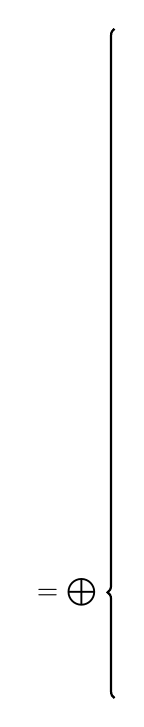
\begin{tikzpicture}
    \draw[decorate,thick,decoration={brace,aspect=0.158}] (0,-8.5) -- (0,0);
    \node[anchor=east] at (-0.1,-7.157) {$= \bigoplus$};
  \end{tikzpicture}%
  \hfill%
  \subcaptionbox{%
    Hierarchical B-splines $\varphi_{l',i'}^p$ ($l' \le l$, $i' \in I_{l'}$)
    and grid points $x_{l',i'}$
    \emph{(dots)}.%
  }[72mm]{%
    \includegraphics{hierarchicalBSpline_2}%
  }%
  \caption{%
    Univariate nodal and hierarchical cubic B-splines ($p = 3$)
    up to level $l = 3$.
    When restricting all functions to $D_l^p$ \emph{(thick black line)},
    the nodal space $V_l^p|_{D_l^p}$ decomposes into the direct sum
    of the hierarchical subspaces $W_{l'}^p|_{D_l^p}$ ($l' \le l$).%
  }
  \label{fig:hierarchicalBSpline}
\end{figure}

In the following, we will only allow odd degrees $p = 1, 3, 5, \dotsc$
in this thesis.
Many theoretical considerations would fail for even degrees.
The basic reason is that for odd degrees, the knots of
$\varphi_{l,i}^p$ coincide with the grid points
\begin{equation}
  x_{l,i-(p+1)/2},\quad
  \dotsc,\quad
  x_{l,i},\quad
  \dotsc,\quad
  x_{l,i+(p+1)/2}.
\end{equation}
For even degrees $p$, the knots of $\varphi_{l,i}^p$ lie exactly in
the middle between two subsequent grid points:
\begin{equation}
  x_{l,i-p/2} - \frac{h_l}{2},\quad
  \dotsc,\quad
  x_{l,i} - \frac{h_l}{2},\quad
  x_{l,i} + \frac{h_l}{2},\quad
  \dotsc,\quad
  x_{l,i+p/2} + \frac{h_l}{2}.
\end{equation}
As we will see in this thesis,
this fact would have many adverse implications.
Most crucial among these are
that the hierarchical splitting \eqref{eq:hierSplittingUV} would not hold,
\todo{insert reference}
that non-uniform hierarchical B-splines would not be able to be defined as
simple as for odd degree,
\todo{insert reference} and
that the so-called fundamental splines would not be defined at all.
\todo{insert reference}
Therefore, and
as these degrees include the hat function case ($p = 1$) and the
most common applied cubic degree ($p = 3$),
it is reasonable to restrict ourselves to odd degrees
for the rest of the thesis.



\subsection{Non-Uniform B-Splines and Proof of the Hierarchical Splitting}

With the hierarchical B-splines $\varphi_{l,i}^p$, we can define
the nodal spaces $V_l^p$ and hierarchical subspaces $W_l^p$
as in \cref{sec:21sparseGrids}.
However, in order for the hierarchical splitting \eqref{eq:hierSplittingUV}
to be correct, we have to prove that the conditions of
\thmref{lemma:hierSplittingUV} are satisfied.
To investigate how the nodal space $V_l^p$ looks like,
we introduce the notion of non-uniform B-splines.

\begin{definition}[non-uniform B-splines]
  \label{def:nonUniformBSplines}
  \newgsymbol{xi!}{$\ß\xi$}{%
    Knot sequence $:= (\xi_0, \dotsc, \xi_{m+p})$%
  }%
  Let $m, p \in \NN_0$ and $\ß\xi = (\xi_0, \dotsc, \xi_{m+p})$ be an
  increasing sequence of real numbers \term{(knot sequence)}.
  \newgsymbol{bkxip}{$b_{k,\ß\xi}^p$}{%
    Non-uniform B-spline of degree $p$ with knots $\ß\xi$ and index $k$%
  }%
  For $k = 0, \dotsc, m - 1$,
  the \term{(non-uniform) B-spline} $b_{k,\ß\xi}^p$ of degree $p$
  with knots $\ß\xi$ and index $k$ is defined by the
  Cox--de Boor recurrence
  \cite{Cox72Numerical,Boor72Calculating,Hoellig13Approximation}
  \begin{equation}
    b_{k,\ß\xi}^p(x)
    :=
    \begin{cases}
      \dfrac{x - \xi_k}{\xi_{k+p} - \xi_k} b_{k,\ß\xi}^{p-1}(x) +
      \dfrac{\xi_{k+p+1} - x}{\xi_{k+p+1} - \xi_{k+1}}
      b_{k+1,\ß\xi}^{p-1}(x),&p \ge 1,\\
      \chi_{\halfopeninterval{\xi_k, \xi_{k+1}}}(x),&p = 0.
    \end{cases}
  \end{equation}
\end{definition}
Note that when choosing $\ß\xi = (0, 1, \dotsc, p + 1)$ and
$k = 0$, we obtain the cardinal B-spline $b^p$.
The definition can be used to characterize the nodal space $V_l^p$:

\begin{proposition}[spline space]
  \label{prop:splineSpace}
  \newgsymbol{Sxip}{$S_\ß\xi^p$}{%
    Spline space of degree $p$ with knots $\ß\xi$%
  }%
  Let $\ß\xi = (\xi_0, \dotsc, \xi_{m+p})$ be a knot sequence.
  Then, the B-splines $b_{k,\ß\xi}^p$ ($k = 0, \dotsc, m - 1$)
  form a basis of the \term{spline space}
  \begin{equation}
    S_\ß\xi^p
    := \spn\{b_{k,\ß\xi}^p \mid k = 0, \dotsc, m - 1\}.
  \end{equation}
  $S_\ß\xi^p$ contains exactly those functions which are continuous
  on $D_\ß\xi^p := [\xi_p, \xi_m]$,
  polynomials of degree $\le p$ on every knot interval
  $[\xi_k, \xi_{k+1}]$ \todo{check half-open interval?} in $D_\ß\xi$
  ($k = p, \dotsc, m - 1$) and at least $(p - 1)$ times
  continuously differentiable at every knot $\xi_k$ in the interior of
  $D_\ß\xi^p$ ($k = p + 1, \dotsc, m - 1$).
\end{proposition}

\begin{proof}
  See \cite{Hoellig13Approximation}.
\end{proof}

This proposition gives the reason for ``B'' in ``B-splines'',
which is for ``basis'' (of the space of splines).
The key observation is that B-splines of a knot sequence $\ß\xi$
do not form a basis of the spline space on the union
$[\xi_0, \xi_{m+p}]$ of the B-spline supports,
but rather on a proper sub-interval $D_\ß\xi^p$.
Intuitively, for every point in $D_\ß\xi^p$ that is not a knot,
exactly $(p + 1)$ B-splines must be \term{relevant} (i.e., non-zero)
to span the spline space as
on every knot interval, the spline is a polynomial of degree $\le p$
and therefore, there must be $(p + 1)$ degrees of freedom.
Outside of $D_\ß\xi^p$, there are too few relevant B-splines
to span the spline space.
This important observation, which is visualized in \cref{fig:splineSpace},
forces us to restrict nodal space and hierarchical subspaces to
$D_\ß\xi^p$:

\begin{figure}
  \includegraphics{splineSpace_1}%
  \caption{%
    Knot sequence $\ß\xi = (\xi_0, \dotsc, \xi_{m+p}$)
    with the corresponding $m = 7$ non-uniform cubic B-splines
    $b_{k,\ß\xi}^p$, $k = 0, \dotsc, m - 1$, $p = 3$.
    On $D_\ß\xi^p$ \emph{(thick line, delimited by dashed lines)},
    which starts with the last knot interval of the first B-spline
    $b_{0,\ß\xi}^p$
    and ends with the first knot interval of the last B-spline
    $b_{m-1,\ß\xi}^p$,
    the B-splines span the spline space $S_\ß\xi^p$.
    Elements of this space are splines $s\colon D_\ß\xi^p \to \RR$
    \emph{(black line)},
    which are linear combinations
    $s = \sum_{k=0}^{m-1} c_k b_{k,\ß\xi}^p$
    of the B-splines.%
  }%
  \label{fig:splineSpace}
\end{figure}

\begin{corollary}[nodal B-spline space]
  \label{cor:nodalBSplineSpace}
  \newgsymbol{f|D}{$f|_D$}{%
    Restriction $f|_D\colon D \to \RR$, $f|_D(x) := f(x)$,
    onto a sub-domain $D$ for a function $f$%
  }%
  \newgsymbol{V|D}{$V|_D$}{%
    Restriction $:= \{f|_D \mid f \in V\}$ onto a sub-domain $D$
    for a function space $V$%
  }%
  \newgsymbol{xilp}{$\ß\xi_l^p$}{%
    Knot sequence for uniform hierarchical B-splines%
  }%
  The restricted nodal B-splines $\varphi_{l,i}^p|_{D_l^p}$
  ($i = 0, \dotsc, 2^l$)
  of level $l \in \NN_0$ are
  a basis of the spline space $S_{\ß\xi_l^p}^p$, where
  \begin{gather}
    \label{eq:nodalBSplineSpaceKnots}
    \xi_{l,k}^p
    := (k - (p+1)/2) h_l,\quad
    k = 0, \dotsc, m + p,\quad
    m := 2^l + 1,\\
    D_l^p := \left[h_l \frac{p-1}{2},\; 1 - h_l \frac{p-1}{2}\right],
  \end{gather}
  and consequently
  \begin{equation}
    V_l^p|_{D_l^p} = S_{\ß\xi_l^p}^p.
  \end{equation}
\end{corollary}

\begin{proof}
  We have $\varphi_{l,i}^p = b_{i,\ß\xi_l^p}^p$ for
  $i = 0, \dotsc, m - 1$,
  as the B-splines on both sides have the same knots.
  The assertions now follow from \thmref{prop:splineSpace}.
\end{proof}

Note that $D_l^p$ might contain only a single point or even be empty,
if $p$ is too large or $l$ is too small.
However, the corresponding B-splines $\varphi_{l,i}^p$ are still linearly
independent on $[0, 1]$ (see \cite{Hoellig13Approximation}).
Similarly, the corollary also implies that the hierarchical functions
$\varphi_{l,i}^p$ ($i \in I_l$) are linearly independent on $[0, 1]$.

\begin{lemma}[first condition of \cref{lemma:hierSplittingUV}]
  The restricted hierarchical subspaces
  $W_{l'}^p|_{D_l^p}$ ($l' \le l$) are
  subspaces of the restricted nodal space $V_l^p|_{D_l^p}$.
\end{lemma}

\begin{proof}
  Every function $\varphi_{l',i'}^p$ ($i' \in I_{l'}$) is continuous on
  $D_l^p$, a polynomial of degree $\le p$ on every knot interval
  of $\ß\xi_l^p$ (due to $p$ odd),
  and at the knots themselves at least $(p - 1)$ times continuously
  differentiable.
  \Cref{prop:splineSpace} implies $\varphi_{l',i'}^p \in S_{\ß\xi_l^p}^p$
  and from \cref{cor:nodalBSplineSpace}, it follows
  $\varphi_{l',i'}^p \in V_l^p|_{D_l^p}$.
  As the functions $\varphi_{l',i'}^p$ ($i' \in I_{l'}$) span
  $W_{l'}^p|_{D_l^p}$, we can conclude
  $W_{l'}^p|_{D_l^p} \subset V_l^p|_{D_l^p}$.
\end{proof}

It is crucial to note that this lemma does not hold for even $p$,
as the knots of the B-splines of level $l - 1$ are not contained in the
knots of level $l$.
This implies that in general,
$W_{l-1}^p|_{D_l^p}$ is not contained in $V_l^p|_{D_l^p}$
for even degrees $p$.
Therefore, the hierarchical splitting equation \eqref{eq:hierSplittingUV}
does not hold, which is the reason for us to restrict the
remaining considerations to odd $p$.

\begin{restatable}[second condition of \cref{lemma:hierSplittingUV}]{%
  proposition%
}{%
  propHierBSplineLinearlyIndependent%
}
  \label{prop:hierBSplineLinearlyIndependent}
  \label{PROP:HIERBSPLINELINEARLYINDEPENDENT}
  The hierarchical B-splines
  $\varphi_{l',i'}^p$ ($l' \le l$, $i' \in I_{l'}$)
  are linearly independent.
\end{restatable}

\begin{proof}
  See \cref{sec:proofHierBSplineLinearlyIndependent}.
\end{proof}

Although we have to restrict all functions and spaces to $D_l^p$,
\thmref{lemma:hierSplittingUV} is still applicable to prove that
the hierarchical splitting equation \eqref{eq:hierSplittingUV}
is correct for hierarchical B-splines:

\begin{corollary}[hierarchical splitting for uniform B-splines]
  \label{cor:hierSplittingBSplines}
  The hierarchical splitting \eqref{eq:hierSplittingUV}
  holds for the hierarchical B-spline basis
  if restricting all functions to $D_l^p$:
  \begin{equation}
    S_{\ß\xi_l^p}^p
    = V_l^p|_{D_l^p}
    = \bigoplus_{l'=0}^l W_{l'}^p|_{D_l^p}.
  \end{equation}
\end{corollary}

\begin{proof}
  Analogously to the proof of \thmref{lemma:hierSplittingUV}
  and apply \thmref{cor:nodalBSplineSpace}.
\end{proof}

This corollary is also visualized in \cref{fig:hierarchicalBSpline}.
We can now proceed to define multivariate
nodal spaces $V_\ßl^p$, hierarchical subspaces $W_\ßl^p$, and
sparse grid spaces $V_{n,d}^{\sparse,p}$ as in \cref{sec:21sparseGrids}.
Note that it is possible to choose different degrees $p_t$ for
different dimensions $t = 1, \dotsc, d$,
since the hierarchical splitting \eqref{eq:hierSplittingMV} does not
require the bases in each dimension to be the same.
Consequently, we can define degree-dimension-adaptive sparse grids
$V_{n,d}^{\sparse,\ßp}$ for arbitrary odd degree vectors $\ßp$.

In the course of this thesis, we will derive multiple variations
of the standard hierarchical B-spline basis.
We will not repeat formal proofs of the hierarchical splitting equation
\eqref{eq:hierSplittingUV}
(i.e., verifying the two conditions of \cref{lemma:hierSplittingUV})
for each of theses bases for the sake of brevity.
The idea of the proof of \cref{prop:hierBSplineLinearlyIndependent},
which is inductively exploiting the smoothness conditions given by
B-splines of previous levels, can often be transferred to similar B-spline
bases.



\subsection{Modification}

Similarly to the piecewise linear case in \cref{sec:213boundary},
Pflüger defined modified
hierarchical B-splines to obtain reasonable values on the boundary
without having to place grid points there \cite{Pflueger10Spatially}.
In \cite{Pflueger10Spatially}, the main motivation is to define basis
functions $\varphi_{l,i}^{p,\modified}$ that satisfy natural boundary
conditions, i.e.,
\begin{equation}
  \label{eq:naturalBoundaryConditions}
  \frac{\diff^2}{\dx^2} \varphi_{l,i}^{p,\modified}(x) = 0,\quad
  x \in \bndry{[0, 1]} = \{0, 1\}.
\end{equation}
Originally, this requirement stems from financial problems
\cite{Pflueger10Spatially}.

For the left boundary,
\eqref{eq:naturalBoundaryConditions} can be satisfied by
modifying the left-most function $\varphi_{l,1}^p$ such that
$\varphi_{l,1}^{p,\modified}(x) = 2 - x/h_l$ is a linear polynomial
when $x$ is ``near'' the boundary.
As in \cite{Pflueger10Spatially},
we append $\varphi_{l,1}^p$ with
B-splines $\varphi_{l,i}^p$ with index $i \le 0$ and
use the so-called Marsden's identity to compute the corresponding
coefficients:

\begin{lemma}[Marsden's identity]
  \label{lemma:marsden}
  Let $p \in \NN_0$ and
  $\ß\xi = (\xi_0, \dotsc, \xi_{m+p})$ be a knot sequence.
  Then, for all $x \in D_\ß\xi^p$ and $y \in \RR$,
  \begin{equation}
    \label{eq:marsden}
    (x - y)^p
    = \sum_{k=0}^{m-1} \big[(\xi_{k+1} - y) \dotsm (\xi_{k+p} - y)\big]
    b_{k,\ß\xi}^p(x).
  \end{equation}
\end{lemma}

\begin{proof}
  See \cite{Hoellig13Approximation}.
\end{proof}

By applying Marsden's identity twice,
\begin{equation}
  2 - \frac{x}{h_l}
  = 2 \sum_{i \in \ZZ} \varphi_{l,i}^p(x)
  - \frac{1}{h_l} \sum_{i \in \ZZ} x_{l,i} \varphi_{l,i}^p(x)
  = \sum_{i \in \ZZ} (2 - i) \varphi_{l,i}^p(x),\quad
  x \in \RR,
\end{equation}
we obtain a possible definition for $\varphi_{l,i}^{p,\modified}$.
Note that only the B-splines with $i \ge 1 - (p+1)/2$
are relevant for the unit interval as all other B-splines vanish in $[0, 1]$.
Pflüger omits summands with $i > 1$ as he only wants to modify
$\varphi_{l,1}^p$ left of its grid point $x_{l,1}$.
The right-most function $\varphi_{l,2^l-1}^{p,\modified}$ can be derived
analogously by mirroring $\varphi_{l,1}^{p,\modified}$ at $0.5$.
For $l = 1$, again the ``constant $1$'' function is taken for the definition
of modified hierarchical B-splines (see \cref{fig:modifiedBSpline}):
\begin{equation}
  \label{eq:modifiedBSplines}
  \varphi_{l,i}^{p,\modified}(x)
  :=
  \begin{cases}
    1,&
    l = 1,\quad i = 1,\\
    \displaystyle\sum_{i'=1-(p+1)/2}^1 (2 - i') \varphi_{l,i'}^p(x),&
    l \ge 2,\quad i = 1,\\
    \varphi_{l,i}^p(x),&
    l \ge 2,\quad i \in I_l \setminus \{1, 2^l - 1\},\\
    \varphi_{l,1}^{p,\modified}(1 - x),&
    l \ge 2,\quad i = 2^l - 1.
  \end{cases}
\end{equation}
By \thmref{prop:splineSpace},
this definition implies that
$\varphi_{l,1}^p(x) = 2 - x/h_l$ ($l \ge 2$)
is only valid for $x \in [0,\; h_l \cdot (5-p)/2]$, i.e.,
the second derivative at $x = 0$ vanishes only for $p \le 5$.
For higher degrees, it is non-zero, albeit very small
in its absolute value.
If it is desired to enforce natural boundary conditions
for higher than quintic degrees,
then the upper bound of $i'$ in the sum in \eqref{eq:modifiedBSplines}
must be extended to $(p+1)/2 - 1$.

\begin{figure}
  \subcaptionbox{%
    Construction of the modified hierarchical cubic B-spline
    $\varphi_{l,1}^{p,\modified}$ (\emph{dashed}, $l \ge 2$)
    as a linear combination of neighboring B-splines $\varphi_{l,i'}^p$
    using Marsden's identity.%
  }[75mm]{%
    \includegraphics{modifiedBSpline_1}%
  }%
  \hfill%
  \subcaptionbox{%
    Modified hierarchical cubic B-splines $\varphi_{l,i}^{p,\modified}$
    and grid points $x_{l,i}$
    \emph{(dots)}.%
  }[75mm]{%
    \includegraphics{hierarchicalBSpline_3}%
  }%
  \caption{%
    Construction of modified hierarchical B-splines and
    the resulting basis.%
  }
  \label{fig:modifiedBSpline}
\end{figure}



\subsection{Non-Uniform Hierarchical B-Splines}

Sparse grid spaces and their corresponding grid point sets,
as we have defined them in \cref{sec:21sparseGrids},
are completely independent of the actual location of the grid points
$x_{l,i}$.
Therefore, it is possible to use different distributions for the grid points
than the standard equidistant choice of $x_{l,i} = i \cdot h_l$,
if the basis functions are altered accordingly.
The so-called Chebyshev points $x_{l,i}^\clenshawcurtis$ and the
resulting Clenshaw--Curtis grids and B-splines will serve as an example.

\newgsymbol{.cc}{$\cdot^\clenshawcurtis$}{%
  Superscript for ``Clenshaw--Curtis (grid point/grid point set/basis
  function/function space/interpolant)''%
}%
The \term{Chebyshev points} $x_{l,i}^\clenshawcurtis$ of level $l \in \NN_0$
are defined as
\begin{equation}
  x_{l,i}^\clenshawcurtis
  := \frac{1 - \cos(\pi x_{l,i})}{2},\quad
  i = 0, \dotsc, 2^l.
\end{equation}
Chebyshev points are the normalized locations of the extrema of the
Chebyshev polynomials $T_{2^l}\colon [-1, 1] \to \RR$,
$T_{2^l}(x) := \cos(2^l \arccos(x))$ \cite{Xu16Chebyshev}.%
\footnote{%
  The literature sometimes uses the name ``Chebyshev points'' for
  the roots of $T_{2^l}$, which are closely connected to the extrema.
  One way to distinguish them is to call the extrema
  ``Chebyshev--Lobatto points'' and the roots
  ``Chebyshev--Gauss points'' \cite{Xu16Chebyshev}.%
}
They are obtained by dividing a semicircle into $2^l$ equally sized
segments and subsequently orthogonally projecting the
segment endpoints onto the diameter
(see \cref{fig:chebyshev}).
The most practical use of Chebyshev points is for
polynomial interpolation to avoid Runge's phenomenon and for
so-called Clenshaw--Curtis quadrature rules.

\begin{figure}
  \includegraphics{chebyshev_1}%
  \caption{%
    Chebyshev points $x_{l,i}^\clenshawcurtis$ on the unit interval $[0, 1]$
    \emph{(black lines)}
    for $l = 0, \dotsc, 4$
    and their construction as the orthogonal projection of the
    endpoints of $2^l$ equally sized segments
    of a semicircle onto its diameter \emph{\textcolor{C0}{(blue)}}.%
  }
  \label{fig:chebyshev}
\end{figure}

In some settings, it can be beneficial to use full or sparse grids consisting
of Chebyshev points, which are then called \term{Clenshaw--Curtis grids},
instead of uniform grids.
Besides the already mentioned advantages for polynomial integration and
quadrature, Clenshaw--Curtis grids can help to reduce interpolation
error in a neighborhood of the boundary of the domain due to the increased
grid point density near the boundary.
If we want to use Chebyshev points as grid points for sparse grids,
we have to employ an appropriate basis to ensure that interpolation
is still possible.
Fortunately, \cref{def:nonUniformBSplines} specifies B-splines for non-uniform
knot sequences.
The \term{hierarchical Clenshaw--Curtis B-spline}
$\varphi_{l,i}^{p,\clenshawcurtis}$ of level $l \in \NN_0$ and index
$i \in I_l$ is defined as
\begin{equation}
  \varphi_{l,i}^{p,\clenshawcurtis}
  := b_{0,\ß\xi_l^{p,\clenshawcurtis}}^p,\quad
  \ß\xi_l^{p,\clenshawcurtis}
  := (x_{l,i-(p+1)/2}^\clenshawcurtis,\; \dotsc,\;
  x_{l,i}^\clenshawcurtis,\; \dotsc,\;
  x_{l,i+(p+1)/2}^\clenshawcurtis),
\end{equation}
where the Chebyshev points $x_{l,i}^\clenshawcurtis$
are equidistantly extended onto $\RR$:
\begin{subequations}
  \label{eq:clenshawCurtisExtend}
  \begin{alignat}{2}
    x_{l,i}^\clenshawcurtis
    &:= i \cdot x_{l,1}^\clenshawcurtis,
    &&\quad i < 0,\\
    x_{l,i}^\clenshawcurtis
    &:= 1 + (i - 2^l) \cdot x_{l,1}^\clenshawcurtis,
    &&\quad i > 2^l.
  \end{alignat}
\end{subequations}
As for the standard hierarchical B-spline basis,
it is now straightforward to define nodal spaces
$V_l^{p,\clenshawcurtis}$
and hierarchical subspaces $W_l^{p,\clenshawcurtis}$ as well as
sparse grid spaces $V_{n,d}^{\sparse,p,\clenshawcurtis}$ and
grid point sets $\Omega_{n,d}^{\sparse,\clenshawcurtis}$
using Cartesian products of Chebyshev points
and tensor products of Clenshaw--Curtis B-splines.
The one-dimensional cubic Clenshaw--Curtis basis and a two-dimensional
sparse Clenshaw--Curtis grid are shown in \cref{fig:clenshawCurtis}.

\begin{figure}
  \subcaptionbox{%
    Hierarchical cubic Clenshaw--Curtis B-splines
    $\varphi_{l,i}^{p,\clenshawcurtis}$ and
    modified Clenshaw--Curtis B-splines
     $\varphi_{l,i}^{p,\clenshawcurtis,\modified}$
    \emph{(dashed)}.%
  }[75mm]{%
    \includegraphics{hierarchicalBSpline_4}%
  }%
  \hfill%
  \subcaptionbox{%
    Sparse Clenshaw--Curtis grid $\Omega_{n,d}^{\sparse,\clenshawcurtis}$
    of level $n = 4$ in $d = 2$ dimensions.%
  }[75mm]{%
    \includegraphics{sg_7}%
  }%
  \caption{%
    Clenshaw--Curtis B-splines and sparse grids.%
  }
  \label{fig:clenshawCurtis}
\end{figure}

Note that in contrast to the standard hierarchical B-spline functions
$\varphi_{l,i}^p$, the Clenshaw--Curtis functions
$\varphi_{l,i}^{p,\clenshawcurtis}$ are not translation-invariant.
As a result, both implementation effort and evaluation runtime
are significantly higher for Clenshaw--Curtis B-splines than
for the standard uniform basis,
as the Clenshaw--Curtis B-splines cannot be precomputed.

Like for uniform B-splines,
\term{modified hierarchical Clenshaw--Curtis B-splines}
$\varphi_{l,i}^{p,\clenshawcurtis,\modified}$ can be defined using the
same method as in \eqref{eq:modifiedBSplines}.
Here, the second derivative does not vanish exactly at the boundary
even for degrees $p \le 5$,
as the formula derived from \thmref{lemma:marsden} assumes uniform knots.
However, as most of the B-spline knots in the summation formula
lie outside $[0, 1]$ and are thus uniformly extended according
to \eqref{eq:clenshawCurtisExtend},
the absolute deviation of the second derivative from $0$ is small.
Again, to enforce the natural boundary condition,
it is possible to recompute the coefficients
of the components $\varphi_{l,i'}^{p,\clenshawcurtis}$
dynamically with Marsden's identity using the correct Chebyshev knots
in \eqref{eq:marsden}.

Please note that our framework permits arbitrary grid point distributions
$x_{l,i}^\ast$,
as long as their number grows exponentially
(i.e., there are $2^l + 1$ points $x_{l,i}^\ast$ in each level $l \in \NN_0$)
and they are nested
(i.e., \eqref{eq:rewriteGridPoint} holds).
Appropriate non-uniform B-spline bases could be defined analogously
to Clenshaw--Curtis B-splines.

\section{Boundary Behavior of Hierarchical B-Splines}
\label{sec:23boundary}

As we have seen in the last section (see \cref{cor:hierSplittingBSplines}),
the hierarchical splitting equation \eqref{eq:hierSplittingUV}
only holds when restricting the function spaces to
$D_l^p = [h_l (p-1)/2,\; 1 - h_l (p-1)/2]$,
which is for $p > 1$ a proper subset of the domain $[0, 1]$.
The implications of this fact on the approximation quality
of the hierarchical B-spline basis are severe.
In this section, we study the underlying reasons of the restriction and
we introduce a new B-spline basis that does not suffer from this issue.



\subsection{Approximation Power of Uniform Hierarchical B-Splines}

Splines are a piecewise generalization of polynomials.
Consequently, approximation spaces spanned by splines of degree $p$ should
at least contain all polynomials of degree $\le p$,
since the approximation power of splines should be at least as good
as that of polynomials.
Unfortunately, this statement is not true for the uniform B-splines
$\varphi_{l,i}^p$ as we have defined them in the last section.
A counterexample is given in \cref{fig:nakInterpolation},
in which a cubic polynomial $f$ is interpolated with
hierarchical cubic B-splines.
However, one can clearly deviations of the interpolant from the polynomial
near the boundary, where the relative error exceeds \SI{10}{\percent}.
The oscillations occur even in the interior of the
spline interpolation domain $D_l^p$.
Of course, this phenomenon does not improve the approximation quality
for other non-polynomial functions as well.

\begin{figure}
  \subcaptionbox{%
    Objective function \textcolor{C0}{$f$ \emph{(blue)}},
    interpolant \textcolor{C1}{$\tilde{f}$ \emph{(red, dashed)}},
    grid points \emph{(dots)}, and
    spline interpolation domain $D_3^p$ \emph{(thick line)}.%
  }[75mm]{%
    \includegraphics{nakInterpolation_1}%
  }%
  \hfill%
  \subcaptionbox{%
    Relative error $|(f - \tilde{f})/f|$ on a logarithmic scale.%
  }[75mm]{%
    \includegraphics{nakInterpolation_2}%
  }%
  \caption{%
    Hierarchical cubic B-splines $\varphi_{l',i'}^p$
    ($l' \le l$, $i' \in I_{l'}$, $p = 3$)
    fail to interpolate the cubic polynomial
    $f(x) := -10.2 x^3 + 14.7 x^2 - 5x + 0.7$
    on the grid of level $l = 3$.%
  }
  \label{fig:nakInterpolation}
\end{figure}

We can explain this as follows:
According to \thmref{cor:hierSplittingBSplines},
we have $S_\ß\xi^p = \bigoplus_{l'=0}^l W_{l'}^p|_{D_l^p}$,
where $\ß\xi$ is as defined in \eqref{eq:nodalBSplineSpaceKnots}
and $p = 3$.
Since cubic polynomials as $f$ are cubic splines as well,
$f \in S_\ß\xi^p$ and, consequently,
$f \in \bigoplus_{l'=0}^l W_{l'}^p|_{D_l^p}$.
This means that there is a linear combination of hierarchical B-splines
$\varphi_{l',i'}^p$ ($l' \le l$, $i' \in I_{l'}$)
that interpolates $f$ exactly on the whole domain $D_l^p$
(not be confused with $\tilde{f}$ in \cref{fig:nakInterpolation},
which does not interpolate $f$ exactly in $D_l^p$).
However, in general, this interpolant is not equal $f$ outside
of $D_l^p$ (i.e., in $[0, 1] \setminus D_l^p$),
as \thmref{prop:splineSpace} only holds for $D_l^p$.
In particular, the interpolant evaluated at $x \in \{0, 1\}$ is not
equal to $f(x)$.
If we now force the additional interpolation conditions in
$x_{l,0} = 0$ and $x_{l,2^l} = 1$,
the resulting interpolant $\tilde{f}$ cannot be the same as the previous
interpolant,
which is why $f$ and $\tilde{f}$ differ inside $D_l^p$.

Formally, the unique existence of an interpolating spline is
described by the so-called Schoenberg--Whitney conditions:

\begin{proposition}[Schoenberg--Whitney conditions]
  Let $\ß\xi = (\xi_0, \dotsc, \xi_{m+p})$ be a knot sequence
  and $t_0, \dotsc, t_{m-1}$ a sequence of interpolation points with
  $\xi_p \le t_0 < \dotsb < t_{m-1} \le \xi_m$.
  Then, there exists a unique interpolating spline
  $s = \sum_{k=0}^{m-1} c_k b_{k,\ß\xi}^p$ for arbitrary data if and only if
  \begin{equation}
    \xi_k < t_k < \xi_{k+p+1},\quad
    k = 0, \dotsc, m - 1.
  \end{equation}
\end{proposition}

\begin{proof}
  See \cite{Hoellig13Approximation}.
\end{proof}

The Schoenberg--Whitney conditions require that the interpolation points
are contained in $D_l^p$.
In the example of $p = 3$ in \cref{fig:nakInterpolation},
the points $0$ and $1$ do not lie in $D_l^p$.
For general degree $p$, the first $(p-1)/2$ and the last $(p-1)/2$
grid points of level $l$ are missing from $D_l^p$,
thus violating the Schoenberg--Whitney conditions.
One possible remedy would be to move these interpolation points inside
$D_l^p$ without changing the corresponding basis functions
(i.e., the knots would stay the same) \cite{Hoellig13Approximation}.
For instance in the cubic case, we could move $0$ and $1$ to
$1.5 h_l$ and $1 - 1.5 h_l$, respectively.
However, with this approach, we would not be able to interpolate
boundary values.
In addition, the condition of the interpolation problem will most likely
worsen if we place interpolation points near the end of the supports
of the corresponding basis functions.

As often, taking slightly a different view of the problem helps
to find a solution.
Let $S_l^p$ denote the space of all splines of degree $p$
on the grid of level $l$, i.e., the space $S_\ß\xi^p$ with
\begin{equation}
  \xi_k := (k - p) h_l,\quad
  k = 0, \dotsc, m + p,\quad
  m := 2^l + p.
\end{equation}
We have $D_\ß\xi^p = [0, 1]$ for this choice of $\ß\xi$, i.e.,
the grid points $x_{l,i}$ ($i = 0, \dotsc, 2^l$) satisfy
the Schoenberg--Whitney conditions for the uniform B-spline basis.
Clearly, $\bigoplus_{l'=0}^l W_l^p$ is a subspace of $S_l^p$,
but it cannot equal $S_l^p$ due to
\begin{equation}
  \dim \bigoplus_{l'=0}^l W_l^p
  = 2^l + 1
  < 2^l + p
  = m
  = \dim S_\ß\xi^p,\quad
  p > 1,
\end{equation}
by \thmref{prop:splineSpace}.
There are too few nodal (and hierarchical) basis functions to
span the whole spline space $S_\ß\xi^p$.

The key idea is now to impose additional $(p - 1)$ boundary conditions
on the basis functions to restrict $S_\ß\xi^p$ to a reasonable subspace
with the correct dimension $(2^l + p) - (p - 1) = 2^l + 1$.
``Reasonable'' means that two requirements should be met:
First, the Schoenberg-Whitney conditions should be satisfied for
the new subspace and the grid of level $l$.
Second, the new subspace should contain all polynomials of degree $\le p$,
eliminating the issue discussed in \cref{fig:nakInterpolation}
in the process.



\subsection{Hierarchical Not-A-Knot B-Splines}

\todo{write}

\blindtext{}



\subsection{Modified and Non-Uniform Hierarchical Not-A-Knot B-Splines}

\todo{write}

\blindtext{}



\subsection{Other Approaches to Incorporate Boundary Conditions}

\todo{write}

\blindtext{}

